\section*{Motivation and Objectives}

%The motivation and objectives section should provide a context for the proposed
%work as well as specific objectives and expected significance of the PhD
%thesis. It should contain a brief overview of the proposed work in relation to
%the present state of knowledge in the field and to work in progress by others.

The Aquapod is proposed as a tool for researchers that will assist with search
and rescue operations as well as the collection of data in a wide array of
terrains.

The Aquapod, \cite{Carlson2011b} \cite{Dhull2012}, is an amphibious small
form-factor robot equipped with a passive buoyancy control unit, embedded
computer capabilities and a wide range of detachable sensing modules that serve
to expand and diversify the capabilites of the robot. The Aquapod has been
designed with the capability to navigate into water from a shoreline and collect
data, such as fluid samples or other sensory data, from a three-dimensional
space bounded by the surface of the body of water and the maximum dive depth.
Utilizing the high mobility-to-size ratio of tumbling locomotion
\cite{Hemes2009} \cite{Hemes2011} as well as the controllable and amphibious
nature of the novel screwdrive powertrain allows movement in both terrestrial
and aquatic environments.


\subsection*{Miniature robotics intro}
% Environmental monitoring 

- Introduction to miniature robotics
- Background (Scout, Adelopod, RC Aquapod)
- Mobility and sensory enhancements for inexpensive miniature robotic platforms.
- Screwdrive and Robotic Locomotion. 
  - Screwdrive design
- Terrainability and Challenges of Screw-Driven Locomotion. 
- Control and Motion Planning Screw-Driven Locomotion.  
- Timeline


\section*{Background}

\subsection*{Miniature robotics}
\subsubsection*{Adelopod, Microvision, Explorer}
\subsubsection*{Aquapod}
\subsection{Aquapod/Adelopod Mobility}

%Following the Deepwater Horizon oil spill in the Gulf of Mexico, several
%methods have been applied to contain the inevitable spread of contaminants.
%In open-water areas, chemical dispersants applied aerially have shown promise
%as a method of response and containment, however, solid and liquid byproducts
%from residual waste that has diffused to coastal areas has proven more
%difficult to address.

%There are several ways to monitor, detect, and analyze the presence of oil
%residues underwater and on the water surface. Skimmers have
%proven effective in collecting oil debris and sheen on the water surface
%\cite{Al-Majed2012}, however, this becomes much more complicated when dealing with
%relatively inaccessible and obstructive terrains, such as those posed by
%marshlands and swamp-like environments. Assessment of toxic chemical
%concentration and collection of fluid samples in these types of conditions can
%be cumbersome.

The Aquapod, a miniature amphibious mobile robot is proposed to assist
environmental scientists and emergency response teams to assess the oil slick
and debris such as that found in the marshes surrounding the Deepwater Horizon
oil spill in the Gulf of Mexicuo. It is an amphibious tumbling robot that presents
high mobility and is capable of navigating terrains which would be difficult
for traditional wheeled platforms. This concept is a continuation of a family
of \emph{tumbling robots} which exhibit a large mobility-to-size ratio, minimalistic
actuation, and high terrainability \cite{Hemes2011, Carlson2011b}. They move on
land by using their arms to create terrain-body interactions that effectuate
end-over-end tumbles.

There are several robotic platforms in development that are capable of both land
and water locomotion.  Such examples are the snake robot AmphiBot I
\cite{Crespi2005b}, the AQUA \cite{Dudek2007b}, or the Whegs\texttrademark IV
\cite{Boxerbaum2005a} which all can traverse both land and sea/underwater
environments with minimal interaction, but are all significantly larger than the
Aquapod and pose a different form factor than this robot.  The aquatic spherical
robot Groundbot \cite{Kaznov2010a} is of similar size and uses terrain-body
interactions as its primary form of locomotion albeit through rolling; however, the
robot was meant to travel soley on the surface of the water, rather than an
underwater environment.  To this end, the Aquapod is intended to be a less
complex alternative to retrieve water samples and collect datat  at varying
depths and return to the surface for recovery, while still allowing superior
mobility relative to its size.

% Bring out to full width size
\begin{figure}[tb]
  \centering
  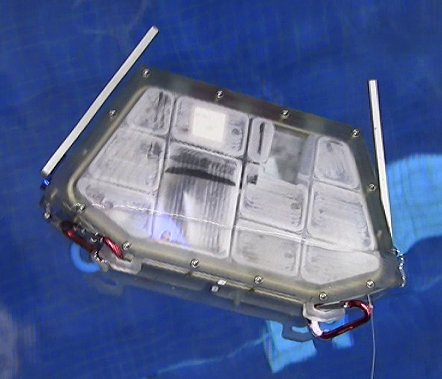
\includegraphics[width=1\columnwidth]{images/100_1800.JPG}
  \vspace{-10pt}
  \caption{Aquapod \cite{Dhull2012}}
  \vspace{-20pt}
  \label{fig:aquapod_pool}
\end{figure}

There are three version of the original Aquapod, or RC Aquapod
~\cite{Carlson2011b}: the RC Aquapod, the Deepwater Horizon Aquapod, and the
Japan Fukushima Aquapod. All these models takes their inspiration from the RC
Aquapod, while revising the design and extending the intended capabilities of
the previous prototype.  The RC Aquapod, in turn, stems from the Adelopod
~\cite{Hemes2011}, using the concept of tumbling for ground locomotion.
However, the Aquapod family adds the ability to function in aqueous
environments, both on the surface and underwater, using a buoyancy control
system to affect its vertical position in the water.  The buoyancy control is a
static alternative to dynamic diving systems used in some submersibles, proving
to be more energy efficient to control the robot's depth by only requiring
energy to change diving characteristics like sinking or floating~
\cite{Detweiler2009a}. This was present in the RC Aquapod, but was
revised and developed in more detail for this application.
%----------------------------------------------------------------------------------------------------------------------------------------------------------


%%%%%%%%%%%%%%%%%%%%%%%%%%%%%%%%%%%%%%%%%%%%%%%%%%%%%%%%%
\section{ Mechanical Design}

Since the RC Aquapod, the mechanical design of almost every component has been
revisited and revised to expand capabilities and design for the environment of a marshland.  It was estimated
that the ``shallow water" environment that the Aquapod was to be used in would
not exceed 10 meters: therefore, the Aquapod was designed to reliably withstand
pressures seen at that depth.  Additionally, energy efficiency was an important
design criteria to ensure a safe recovery of the robot, thus the Aquapod uses a
peristaltic pump and a bladder to ingest surrounding water to alter its
buoyancy.  This system was present in the RC Aquapod, but was revised and
developed in more detail to meet the specified design requirements, notably the
chemical compatibility of components that interact with the environment.

The outer shell of the Aquapod is made out of clear polycarbonate, which meets
both the stress requirements for diving to 10 meters and is chemically
compatible with materials that the Aquapod is expected to encounter.  Among the
major challenges and additions to the Aquapod design, is the new sealing
methodology including all connections and seams in the hull--which encloses the
electronics, the revision of the Buoyancy Control Unit (BCU), the revisited
drive system for the arms, as well as the addition of an external water sampling
module attaching directly to the outer hull of the robot. See Figure
\ref{fig:annotated_aquapod} for a diagram of the internal components.

  \subsubsection{Sealing} In order for the Aquapod to be capable to descend to
  designed depth, all locations susceptible to fluid ingression were designed to
  withstand a maximum hydrostatic gauge pressure of approximately 14 psi\(_g\),
  double that of atmospheric pressure.

% Main seal
    The seal formed between the top and bottom halves of the hull, the main
    seal, is formed by compression of an O-ring. This seal was designed to be
    hermetic and withstand the maximum design pressure.  Empirical results found
    this particular seal to have greater performance over alternate designs,
    including the flat-gasket design of the RC Aquapod.

    \begin{figure}[htb]
      \centering
      %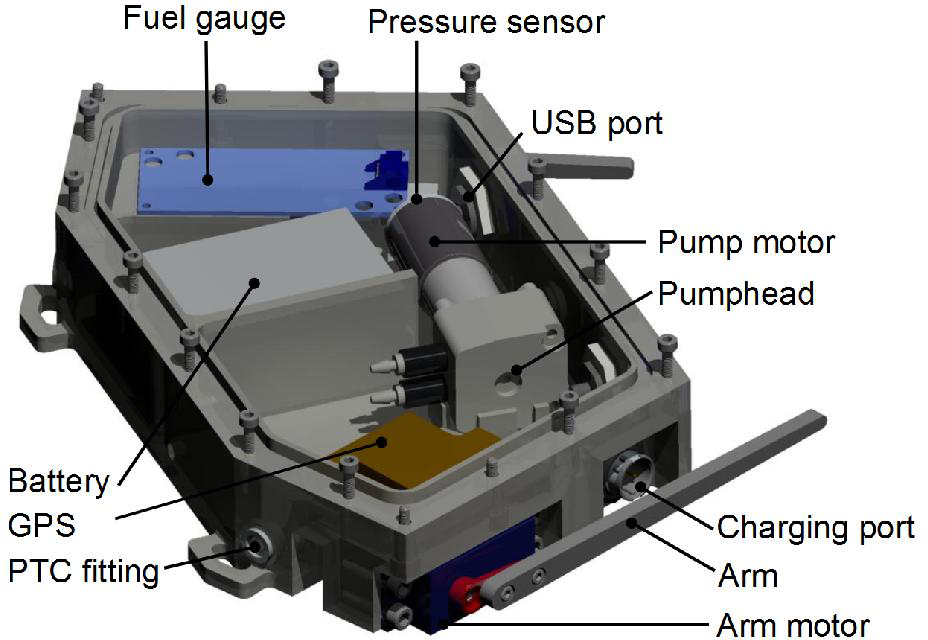
\includegraphics[width=.90\columnwidth]{images/Aquapod2-Mod.png}
      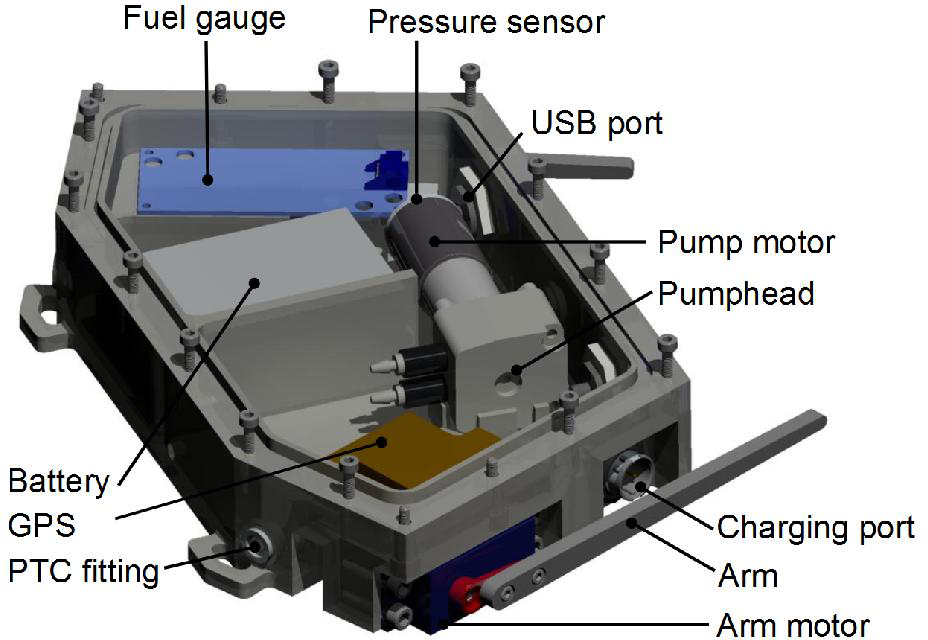
\includegraphics[width=.90\columnwidth]{images/Aquapod2-Mod.pdf}
      \caption{Aquapod components}
      \vspace{-20pt}
      \label{fig:annotated_aquapod}
    \end{figure}


    One of the main advantages of the O-ring and gland design was lower force
    requirements to form an effective seal than other designs. This is
    advantageous because the seal is highly dependent on the compressive force
    exerted between the hull halves, however, the maximum force that was
    exertable is a function of the stress that the material and fastening method
    allow. Polycarbonate was chosen for the hull material and the hulls were
    fastened by a set of screws on the periphery of the Aquapod, therefore
    minimal compression force requirements were necessary to prevent stripping
    out the threads of the tapped holes.

    Another advantage of the O-ring is that it forms a more robust seal as its
    circular cross-section provides a sealing profile that commences with linear
    contact and progresses to an area as the O-ring is compressed. This initial
    linear contact is desirable because it concentrates greater sealing pressure
    at the onset of the sealing phase. The alternative gasket design, required
    special features, such as a tooth, to be incorporated into the hull, to form
    an effective seal.  This method presented its own challenges, as high
    compressive forces were required, but over compression can lead to rupture
    of the gasket.

    Other locations that were susceptible to fluid ingression include various
    ports, power components, the external motors, and lines that provided power
    and communication to the external motors. The pressure sensor port is
    press-fit into the hull and sealed in conjunction with a
    tetrachloroethylene-based marine sealant and adhesive (herein referred to
    simply as sealant). The Aquapod sports two commercial-off-the-shelf (COTS)
    mini-USB panel-mounted ports for data I/O as well as for programming.  These
    ports are desirable as compatible hardware is easily found and convenient.
    The ports are Ingress Protection 68 (IP68) rated and were modified to extend
    their sealing capabilities to meet our specification requirements.

    The power switch is a double-pole double-throw three position micro-switch
    with a rubber boot to ensure hermeticity. Power components include the
    on/off switch and the charging ports, these were COTS and were implemented
    in the design with no further modifications.

    The control and power buses for the arms and the sampler module servos, are
    routed through flexible PVC tubing in order to take advantage of industry
    standard pneumatic push-to-connect (PTC) fittings.  The PTC fittings form a
    hermetic seal with the tubing and their design prevents accidental
    disconnection by unexpected tension, e.g.\ when a twig or other obstacle
    become caught on the tubing. The sealing of the external motors will be
    described in Section \ref{arm_motors} below.

  \subsubsection{Buoyancy Control Unit} The BCU is largely similar to the one
  used in the RC Aquapod. It is comprised of a bladder, gearmotor, and pumphead.
  The current iteration of the BCU has seen the addition of an encoder for
  angular velocity feedback as well as a motor specified to meet greater torque
  and angular velocity requirements while also meeting weight and volumetric
  constraints.  Additionally, the stock tubing in the pumphead was replaced with
  one that offers high chemical compatibility with fluids which it could
  potentially contact while minimizing the hardness of the tube to achieve
  higher flowrates.

  \subsection{Chemical Compatibility} The Aquapod was intended as a tool to
  assist in environmental monitoring, therefore, the hull, main seal, and all
  other surfaces exposed to the potential chemical-laden environments need to be
  chemically compatible with substances that may negatively impact their
  properties. A short list of fluids that were taken into account consist of
  fresh water, salt water, crude oil, gasoline, diesel fuel, and fuel oils.

  A material's chemical compatibility was one of the most important factors
  when choosing components that would be in contact with external fluids.
  The severity of foreign chemicals on the elastomeric components is a
  function of concentration as well as time with the main consequences being
  swelling or stiffening of the elastomers.

  The bladder, O-ring, and tubing were the components most susceptible to
  chemical degradation, therefore the selection of these components was in
  large part driven by compatibility constraints. The O-ring is made of a
  formulation of Viton\textsuperscript{\textregistered} that is compatible
  with the aforementioned fluids and has 40 Shore A hardness which creates a
  better seal in low pressure applications \cite{Seals2007}.

  The pump is one of the components that is most susceptible to the potential
  degradation due to the elastomeric tubing which forms part of its design and
  serves to transport fluids. These fluids originate exterior to the Aquapod
  and are potential carriers of chemicals that can degrade the tubing. The
  peristaltic pumphead constrains and squeezes sections of tubing to provide
  fluid displacement. Chemical degradation can aggravate the significant
  stress already imparted on the tubing mechanically and lead to premature
  failure.

  Tubing hardness is important as the flowrate is inversely proportional to
  the tubing hardness. The silicone tubing that comes stock with the pumphead
  offers a favorable flowrate; however, due to its poor chemical
  compatibility, it was replaced with unreinforced high-flex white PVC.  The
  PVC tubing meets chemical compatibility constraints and has approximately
  the same hardness as the stock silicone tubing.

  \subsubsection{Arm Powertrain} \label{arm_motors} The Aquapod's powertrain is
  found completely external to the hull and consists of a set of motors on the
  underside of the robot that are coupled to a pair of aluminum arms. The
  Aquapod moves by driving arms to execute end-over-end tumbles. To achieve
  forward motion on flat terrain, the arms move in unison in the same direction,
  however, in order to move in nonuniform terrain or other types of movements it
  was desirable to exploit the differential nature of the powertrain. Situations
  arise in which, due to the terrain, or the required type of movement only one
  arm is used to move the robot.  Therefore it was necessary to specify the
  powertrain to meet scenarios in which the Aquapod's weight relies solely on
  one arm and motor.

    The geometry of the Aquapod's arms were driven primarily by the need to
    support the full weight of the Aquapod (approximately 2.65 lbs) to enable
    effective tumbling. Material selection was important in choosing a material
    of low weight and high resistance to corrosion in marine environments, as
    well as meet the chemical compatibility requirements from the previous
    section.

    The Aquapod's arms are driven by high torque servomotors that have been
    modified for hermeticity and continuous rotation. Enabling continuous
    rotation from an COTS servomotor required mechanically altering the output
    gear of the geartrain, replacing the stock circuitry with an analog absolute
    encoder capable of providing an analog output for continuous position
    feedback, and providing control via the onboard embedded system.

    Ensuring hermeticity after arm motor modifications presented multiple
    sealing challenges.  The motors' stock configuration features a rubber
    grommet that routes three wires through its exterior housing.  In light of
    the addition of the encoder, it was necessary to route two additional wires
    through the shell, bringing the total to five.  The wires are routed inside
    soft PVC tubing which acts as the new grommet. Routing the power and control
    buses in tubing also allows an effective seal using the PTC fittings found
    on the hull. Additionally, using a combination of tubing and fittings allows
    the arm servos to be easily replaced. The new grommet and the seams present
    throughout the exterior motor housing are further sealed with marine
    sealant.

  The most critical seals of the Aquapod are located at the output shafts of the
  arm motors as these seals are dynamic in nature. Being dynamic they require a
  seal to be kept when the powertrain is in motion. The motor's stock
  configuration contains a bearing and O-ring that are mounted on the output
  shaft of the arm servo. The bearing serves to align the output shaft and the
  O-ring to form a seal with the exterior motor housing. To improve seal
  pressure the stock O-ring was replaced with a thicker and softer Buna-N
  O-ring. Additionally, exterior to the motor housing, an O-ring was added to
  form a secondary seal when compressed between the external housing and the
  arm.

  \subsubsection{Sampler Design} The sampler module was designed and created for
  the Aquapod in order to capture water samples and bring them to the surface.
  Equipment utilized to carry out substance detection methods are not practical
  in miniature robots, therefore, collecting these samples is valuable.
  Furthermore, a more thorough analysis of the samples can be done in a
  laboratory setting.

Figure~\ref{fig:sampler} shows a rendering of the sampler module which attaches
to the backside of the Aquapod.  The module is designed with energy efficiency
in mind to prolong battery life: thus, two caps on each end of a tube are held
closed by an elastic band requiring no electric power to remain closed.  A servo
is engaged only to open each end and take the sample, then released to close the
vials again.  The caps are padded with a rubber surface, while the tubes have
been filed to a sharper end to promote higher pressure between the tube and the
caps (by reducing the contact area) and thus more effectively sealing the vial.

The current model has two vials, each opened by its own servomotor.  The motors
themselves required additional modifications to survive the maximum design
pressure: marine sealant was applied to each seam in the plastic body, a thicker
O-ring was placed on the shaft of the servo to seal it, and the circuitry inside
the servo was covered in epoxy. This substantially improved the life of these
units.

A waterproof connector runs into the hull of the Aquapod to connect power and
signal lines to the interior electronics.  These connectors are also injected
with epoxy to ensure a waterproof connection.  The backpack itself is attached
to the Aquapod hull using screws for easy removal.

\begin{figure}[htb]
  \centering
  \includegraphics[width=1\columnwidth]{images/sample_v2.pdf}
  \caption{Sampler}
  \vspace{-10pt}
  \label{fig:sampler}
\end{figure}
%----------------------------------------------------------------------------------------------------------------------------------------------------------

%%%%%%%%%%%%%%%%%%%%%%%%%%%%%%%%%%%%%%%%%%%%%%%%%%%%%%%%%%%%%%%%%%%%%%%%%%%%%%%%%%%%%%%%%%%%
%\section{Embedded System Design} This section presents an overview of the
%embedded system design of the Aquapod, which has been split into three main
%components. Two of the printed circuit boards (PCBs) were custom designed to
%meet the volume restrictions while the third PCB was a small, COTS module.
%Splitting the electronics into separate boards allows the design to be highly
%versatile and expand with minimal effort. This also allowed for different sensor
%suites to be interchanged and made the robot more robust to ever adapting needs.

%%%%%%%%%%%%%%%%%%%%%%%%%%%%%%%%%%%%%%%%%%%%%%%%%%%%%%%%%%%%%%%%%%%%%%%%%%%%%%%%%%%%%%%%%%%%
%\subsubsection{Hardware Design} The initial RC Aquapod had no embedded system
%design, and so the new iteration had to make a number of drastic changes. Due to
%the increase in internal components, space inside the robot was limited. A
%three-PCB design made up of a master board, a slave board, and a fuel-gauge
%board allowed the components to be broken apart and better utilize the space
%available. The complete system architecture can be seen in Figure
%\ref{fig:final-arch}.
%
%\begin{figure}[ht]
  %\begin{center}
    %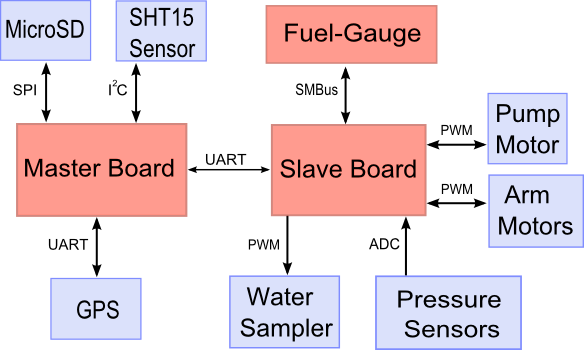
\includegraphics[width=1\columnwidth]{images/finalized-architecture2.png}
    %\caption{Final embedded system architecture}
    %\vspace{-20pt}
    %\label{fig:final-arch}%
  %\end{center}
%\end{figure}

%%%%%%%%%%%%%%%%%%%%%%%%%%%%%%%%%%%%%%%%%%%%%%
%\subsubsection{Master Board} In order to facilitate the requirements within the
%time constraints, a COTS module was used for the master board. SparkFun
%Electronics sells this as the Package Tracker and runs on an LPC2148 ARM7
%microcontroller. This unit was chosen for its 'ready to use' mircoSD card
%reader, onboard sensors, and GPS interface.  The master board is responsible for
%controlling the state machine of the robot, making decisions, and logging the
%sensor data.

%\subsubsection{Slave Board} Due to the custom nature of the hardware, the slave
%board was designed specifically for the Aquapod robot. The main processor was
%chosen as the PIC16F1827 from MicroChip based on the number of required input
%and output pins. The slave board also includes a pressure sensor, charge
%recognition circuitry, communication devices, and the required motor drivers for
%five separate actuators (two arms, two samplers, and one pump). This board
%facilitates the low-level control of the motors and sensors, however, it will
%only act on commands sent by the master board.

%%%%%%%%%%%%%%%%%%%%%%%%%%%%%%%%%%%%%%%%%%%%%%
\subsubsection{Sensors} The Aquapod has two absolute pressure sensors with an
output range of 0.3V to 4.9V, corresponding to an input range of 3 psi\(_a\) to
42 psi\(_a\), respectively. These sensors are used to monitor internal and
external pressure and act as the main decision points of the state machine.

The two arm motors feature absolute magnetic shaft encoders to report the
current arm position back the slave board which handles the PID control for arm
movement. The pump motor also includes a digital encoder to determine the total
water volume pumped into the bladder. The sampler motors have no feedback, but
operate on a standard servo open-loop signal.

The COTS master board contains a number of onboard sensors including
temperature, humidity, and a 3-axis accelerometer. The board can also access the
SiRF III GPS module from USGlobalSat.

By communicating with the slave board, the master board is capable of measuring
and logging all of these sensor values in a central log file and can make
decisions based on the returned values, this will be discussed in more detail
below.
%%%%%%%%%%%%%%%%%%%%%%%%%%%%%%%%%%%%%%%%%%%%%%
%\subsection{Power Architecture} The Aquapods's power system comprises of
%three main parts: the battery and fuel-gauge, the battery charger, and the
%various power conversion electronics.  Wiring to chassis-mounted electronic
%components and high DC current lines is realized using twisted-pairs to increase
%noise immunity by reducing destructive (or unbalanced) effects resulting from
%electromagnetic interference coupled signals and ground return paths.

%\subsubsection{Battery and Fuel-Gauge}
%\label{sec:batt_mgmt_and_gg}
%At the heart of the robot's power system is a dedicated fuel-gauging chipset,
%described in \cite{Kottas2009}.  It provides all the necessary features to
%safely monitor any lithium-ion battery chemistry's dynamics, while tracking cell
%(capacity) degradation over time.  The resultant smart-battery system (SBS) is
%compliant with SBS v1.1 standards and can report a wide array of
%static and dynamic battery parameters while idle, charging, or discharging to a
%host processor - in this case, the slave and master boards. This system is shown
%in Figure \ref{fig:pwr_blk_diag}.
%
%A lithium-ion polymer battery (LiPB) was chosen to power the robot.  This
%particular battery chemistry was selected due to its thin and light-weight
%packaging, high energy density and output power capabilities.  It can source
%roughly 14Wh of energy, and satisfies the robot's operating time requirements.
%
%A highly integrated LiPB switch-mode charge-management circuit is included on
%slave board.  It is configured to charge the LiPB pack quickly and safely and
%contains a pre-charge (conditioning) mode for deeply discharged batteries.
%
%\begin{figure}
  %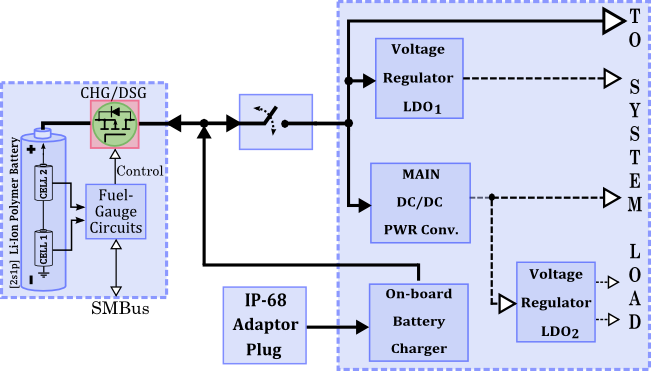
\includegraphics[width=1\columnwidth]{images/Aqua-Pod_Robot_PwrSys_Fig01.png}
  %\caption{High-level power system block diagram}
  %\vspace{-10pt}
  %\label{fig:pwr_blk_diag}
%\end{figure}
%
%%%%%%%%%%%%%%%%%%%%%%%%%%%%%%%%%%%%%%%%%%%%%%
%\subsubsection{Communication Protocol} Command and Acknowledgment (CMD/ACK)
%messages are used to exchange data and commands between the boards. This
%hand-shaking protocol was enforced to ensure important commands from the master
%board were being process and executed by the slave board before continuing with
%the state machine. The master board can send one command at a time in a 9-byte
%packet to the slave board which will execute the command or return sensor values
%appropriately.
%%%%%%%%%%%%%%%%%%%%%%%%%%%%%%%%%%%%%%%%%%%%%%%
%\subsection{State Machine and Operational Profiles} The main purpose for this
%version of the Aquapod was to collect water samples at a pre-programmed depth.
%Using a graphical user interface, the Aquapod can be programmed into one of four
%modes, including: Instant Dive(1), Remote Dive(2), Land Mode(3), and Purge
%Bladder(4). Selecting one of these modes will route the robot through the state
%machine which can be seen in Figure \ref{fig:Statemachine}.
%
%\begin{figure}
  %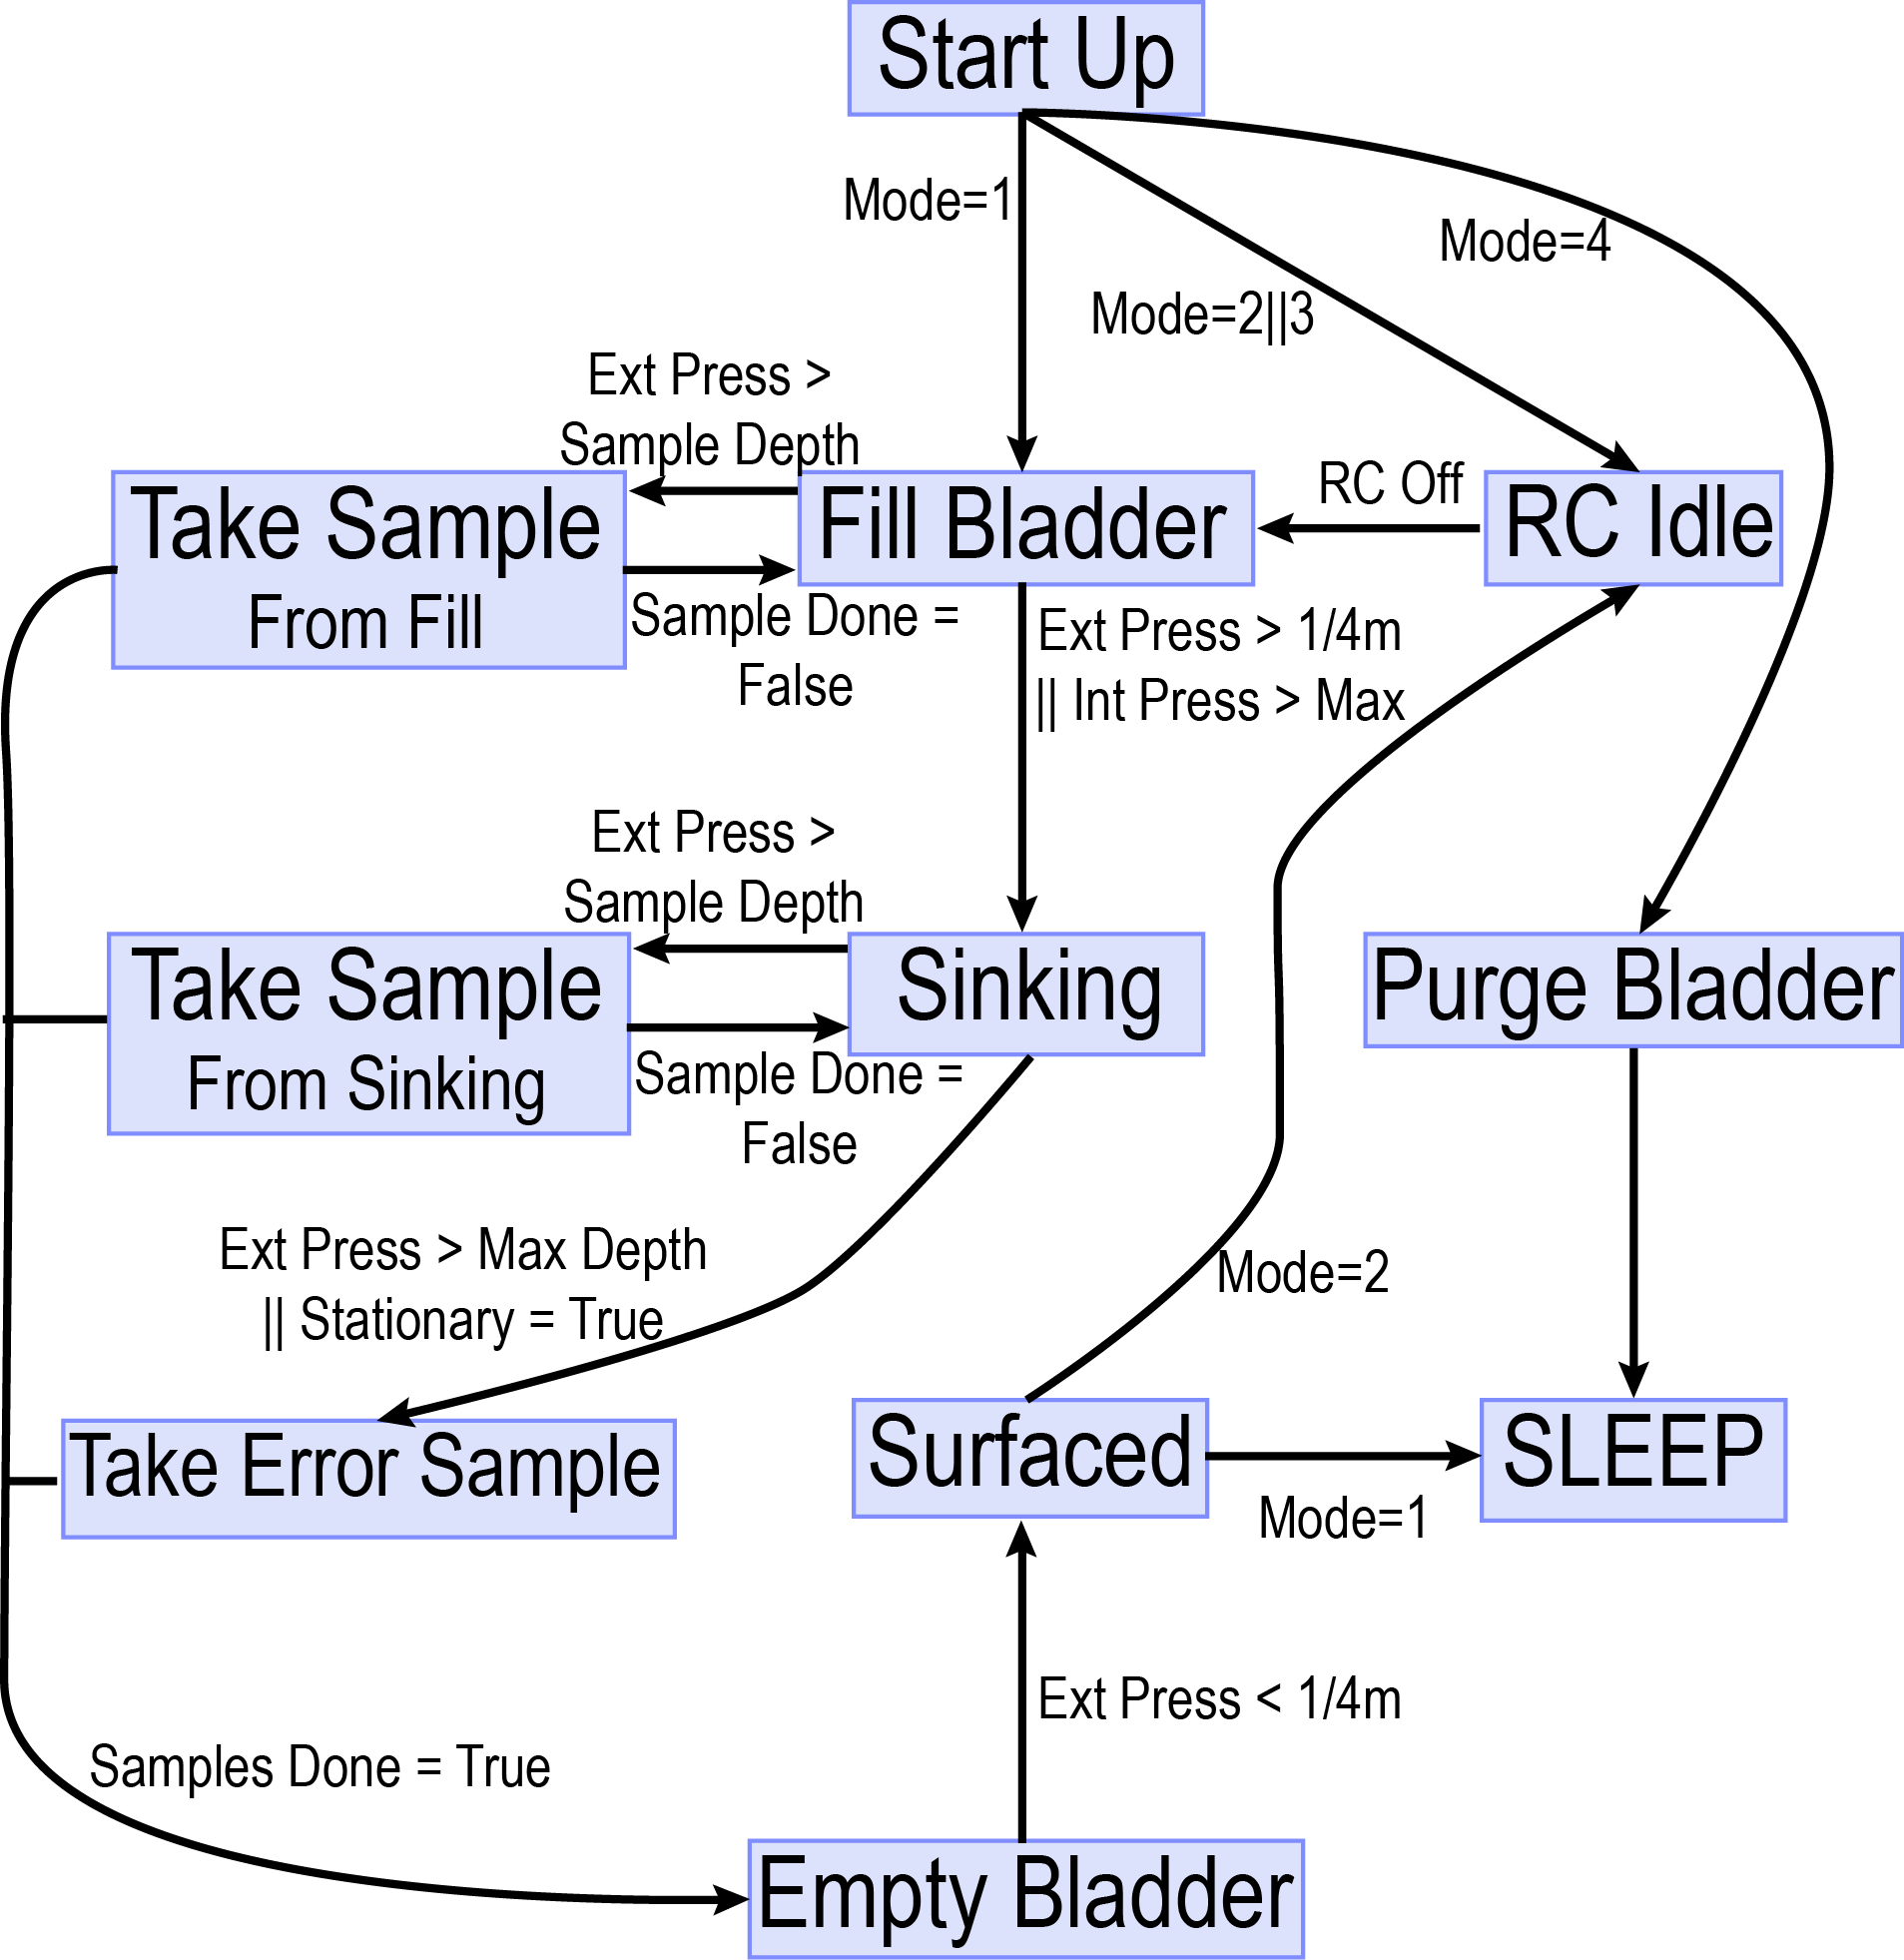
\includegraphics[width=1\columnwidth]{images/Statemachine.png}
  %\caption{Aquapod state machine diagram}
  %\vspace{-10pt}
  %\label{fig:Statemachine}
%\end{figure}
%
%It was important to program a number of safety checks within the state machine
%to ensure that the robot will always resurface. Errors in the operation could
%include reaching a depth greater than 10m or hitting a surface before reaching
%the target depth. If one of these errors occurs, the robot will take a sample
%and return to the surface. Other system error checks were written directly into
%the slave board in case one of the boards reset, a sensor failure occurs, or
%other unlikely mishaps happen.
%
%During either mode 2 or 3, the remote control (RC) operation is run. This allows
%the user to control the arms of the robot through a standard radio transmitter.
%In these modes the user can command the robot to tumbling to a particular
%location and dive or simply move around on land.  ub The state machine featured
%in Figure \ref{fig:Statemachine} is by no means extensive of the robot's
%capabilities. Further development and inclusion of the GPS module can greatly
%increase the functionality of the robot. This operation profile was simply used
%as an example for diving/sampling and as a demonstration tool. Autonomous
%control for long-term and unmonitored missions is feasible with the current
%hardware.
%
%%%%%%%%%%%%%%%%%%%%%%%%%%%%%%%%%%%%%%%%%%%%%%%%%%%%%%%%%%%%%%%%%%%%%%%%%%%%%%%%%%%%%%%%%%%%%
%\subsection{Experiments} \label{experiments}
To verify the mechanical design and
embedded system programming, numerous experiments were carried out in a diving
well. Figure \ref{fig:logfile} shows the results from a sample dive that was
aken. The robot was programmed to take samples at 1m and 3m. The output log
file includes the internal pressure values, depth in meters, the accelerometer
ensors, temperature, and humidity. Markers are placed on the pressure graph to
indicate event locations either the pump turning on or off(solid), or when a
sample was taken(dotted).

\begin{figure}[htb]
  \centering
  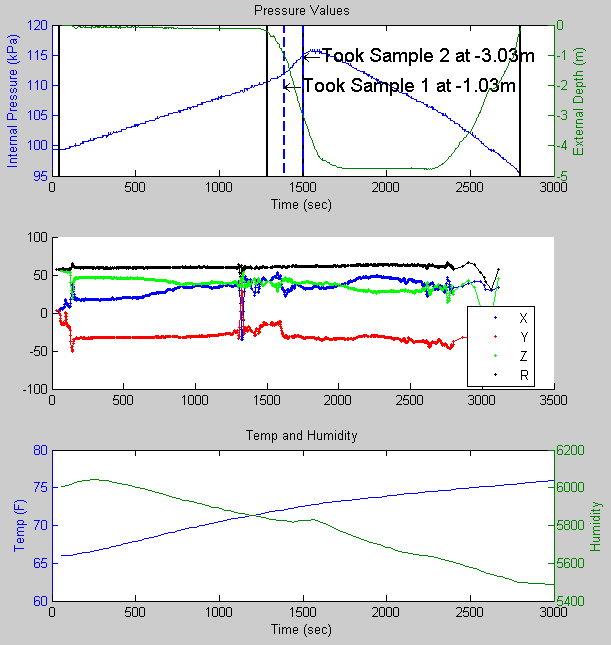
\includegraphics[width=1\columnwidth]{images/logfile.png}
  \caption{Experiment log file from an Aquapod dive} \vspace{-10pt}
  \label{fig:logfile}
\end{figure}

In addition to in-lab testing, the Aquapods were also brought to Houston for
user testing with research biologists. The robots were demonstrated in several
locations in marshlands near the coast including heavily vegetated and muddy
environments. Feedback from this visit will be taken into consideration for
future iterations of the Aquapod family.

%%%%%%%%%%%%%%%%%%%%%%%%%%%%%%%%%%%%%%%%%%%%%%%%%%%%%%%%%%%%%%%%%%%%%%%%%%%%%%%%%%%%%%%%%%%%
%\subsection{Future Work} \label{future_work} Though this iteration was a major
%improvement in functionality over the pervious RC Aquapod, many improvements are
%continously being explored to expand its capabilities. One area of continuing
%work for the Aquapod is communications. Currently the only method of
%communication is through hobby RC signals. However, Aquapods can be configured
%to carry distinct communication payloads, with each Aquapod serving as a node in
%a network that enables digital radio, cellular, and acoustic communications.
%
%Improvements to the electrical power system design include the use a single-cell
%LiPB. This broadens the range of compatible input power sources to include
%various energy harvesting modules - such as solar, wave, thermal, kinetic, etc.
%Integrating dynamic power-path management into the charging circuit, in tandem
%with energy harvesting may also increase efficiency of energy use achieving
%overall gains in the robot's achievable runtime.
%
%Another improvement relates to using the Aquapod for extended-period
%environmental monitoring. In this scenario, the robot collects relevant data in
%a manner that minimizes energy consumption for periods of 12 to 24 hours and
%then navigates to a waypoint for pickup.

%%%%%%%%%%%%%%%%%%%%%%%%%%%%%%%%%%%%%%%%%%%%%%%%%%%%%%%%%
%\section{ Conclusions}
%
  %The combination of the high terrainability, high mobility-to-size ratio,
  %amphibious nature, and small size allows the deployment of the Aquapod in
  %environments that would be difficult for most robots of the same size. The
  %robot is designed to withstand water pressures up to 10 meters in depth, as
  %well as be chemically compatible with the potential substances it may
  %encounter.  The onboard embedded system was designed to perform as many
  %modular expandable tasks in a limited amount of space, as well as provide
  %intelligent power management to the system.  The redesign and further
  %development of this robotic platform provided several advances in its
  %capability for the specified environment of a shallow water marshland.
%%
%
%


%\subsection{Aquapod}

%\subsection{ICRA 2017} source

The Aquapod from the Center for Distributed Robotics is an amphibious robotic
platform that leverages tumbling locomotion to overcome obstacles that are large
relative to its size. It is fully waterproof up to 10 meters allowing it to
traverse land, amphibious, or fully aquatic environments.

The Aquapod has a passive buoyancy control unit that works by ingesting a fluid,
in this case water, and changing its density thereby altering its buoyancy
\cite{Carlson2011b}. The change in buoyancy enables the robot to ascend and
descend in a body of water all while using less resources than a comparable
active buoyancy control unit or active propulsion in general \cite{Dhull2012}.

Embedded in this robotic platform are a suite of pressure, temperature, and
conductivity sensors. Additionally a GPS unit is installed and wireless
connectivity is provided for programming and data extraction using the 802.11
and 802.14 protocols and necessary hardware.

These robotic platforms are expected and designed to work in a myriad of
environments and overcome unforeseen obstacles in the environment leveraging its
waterproof nature, high terrainability \cite{Hemes2011}, and extensibility.
Despite a minimal amount of hardware complexity the Aquapod is able to achieve a
high mobility-to-size ratio enabling negotiation of a variety of complex terrain
where conventional forms of robotic locomotion would fail.

\begin{figure}[!ht] \centering
  %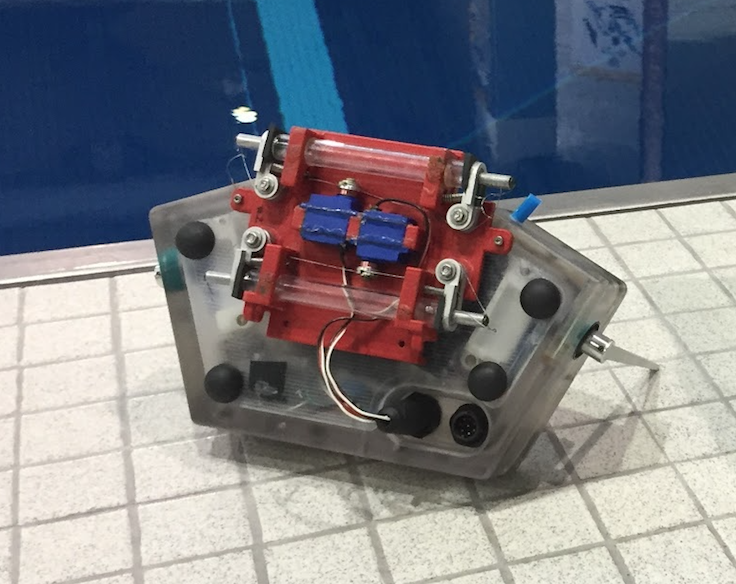
\includegraphics[width=1\columnwidth]{images/aquapod_sampler_well.png}
  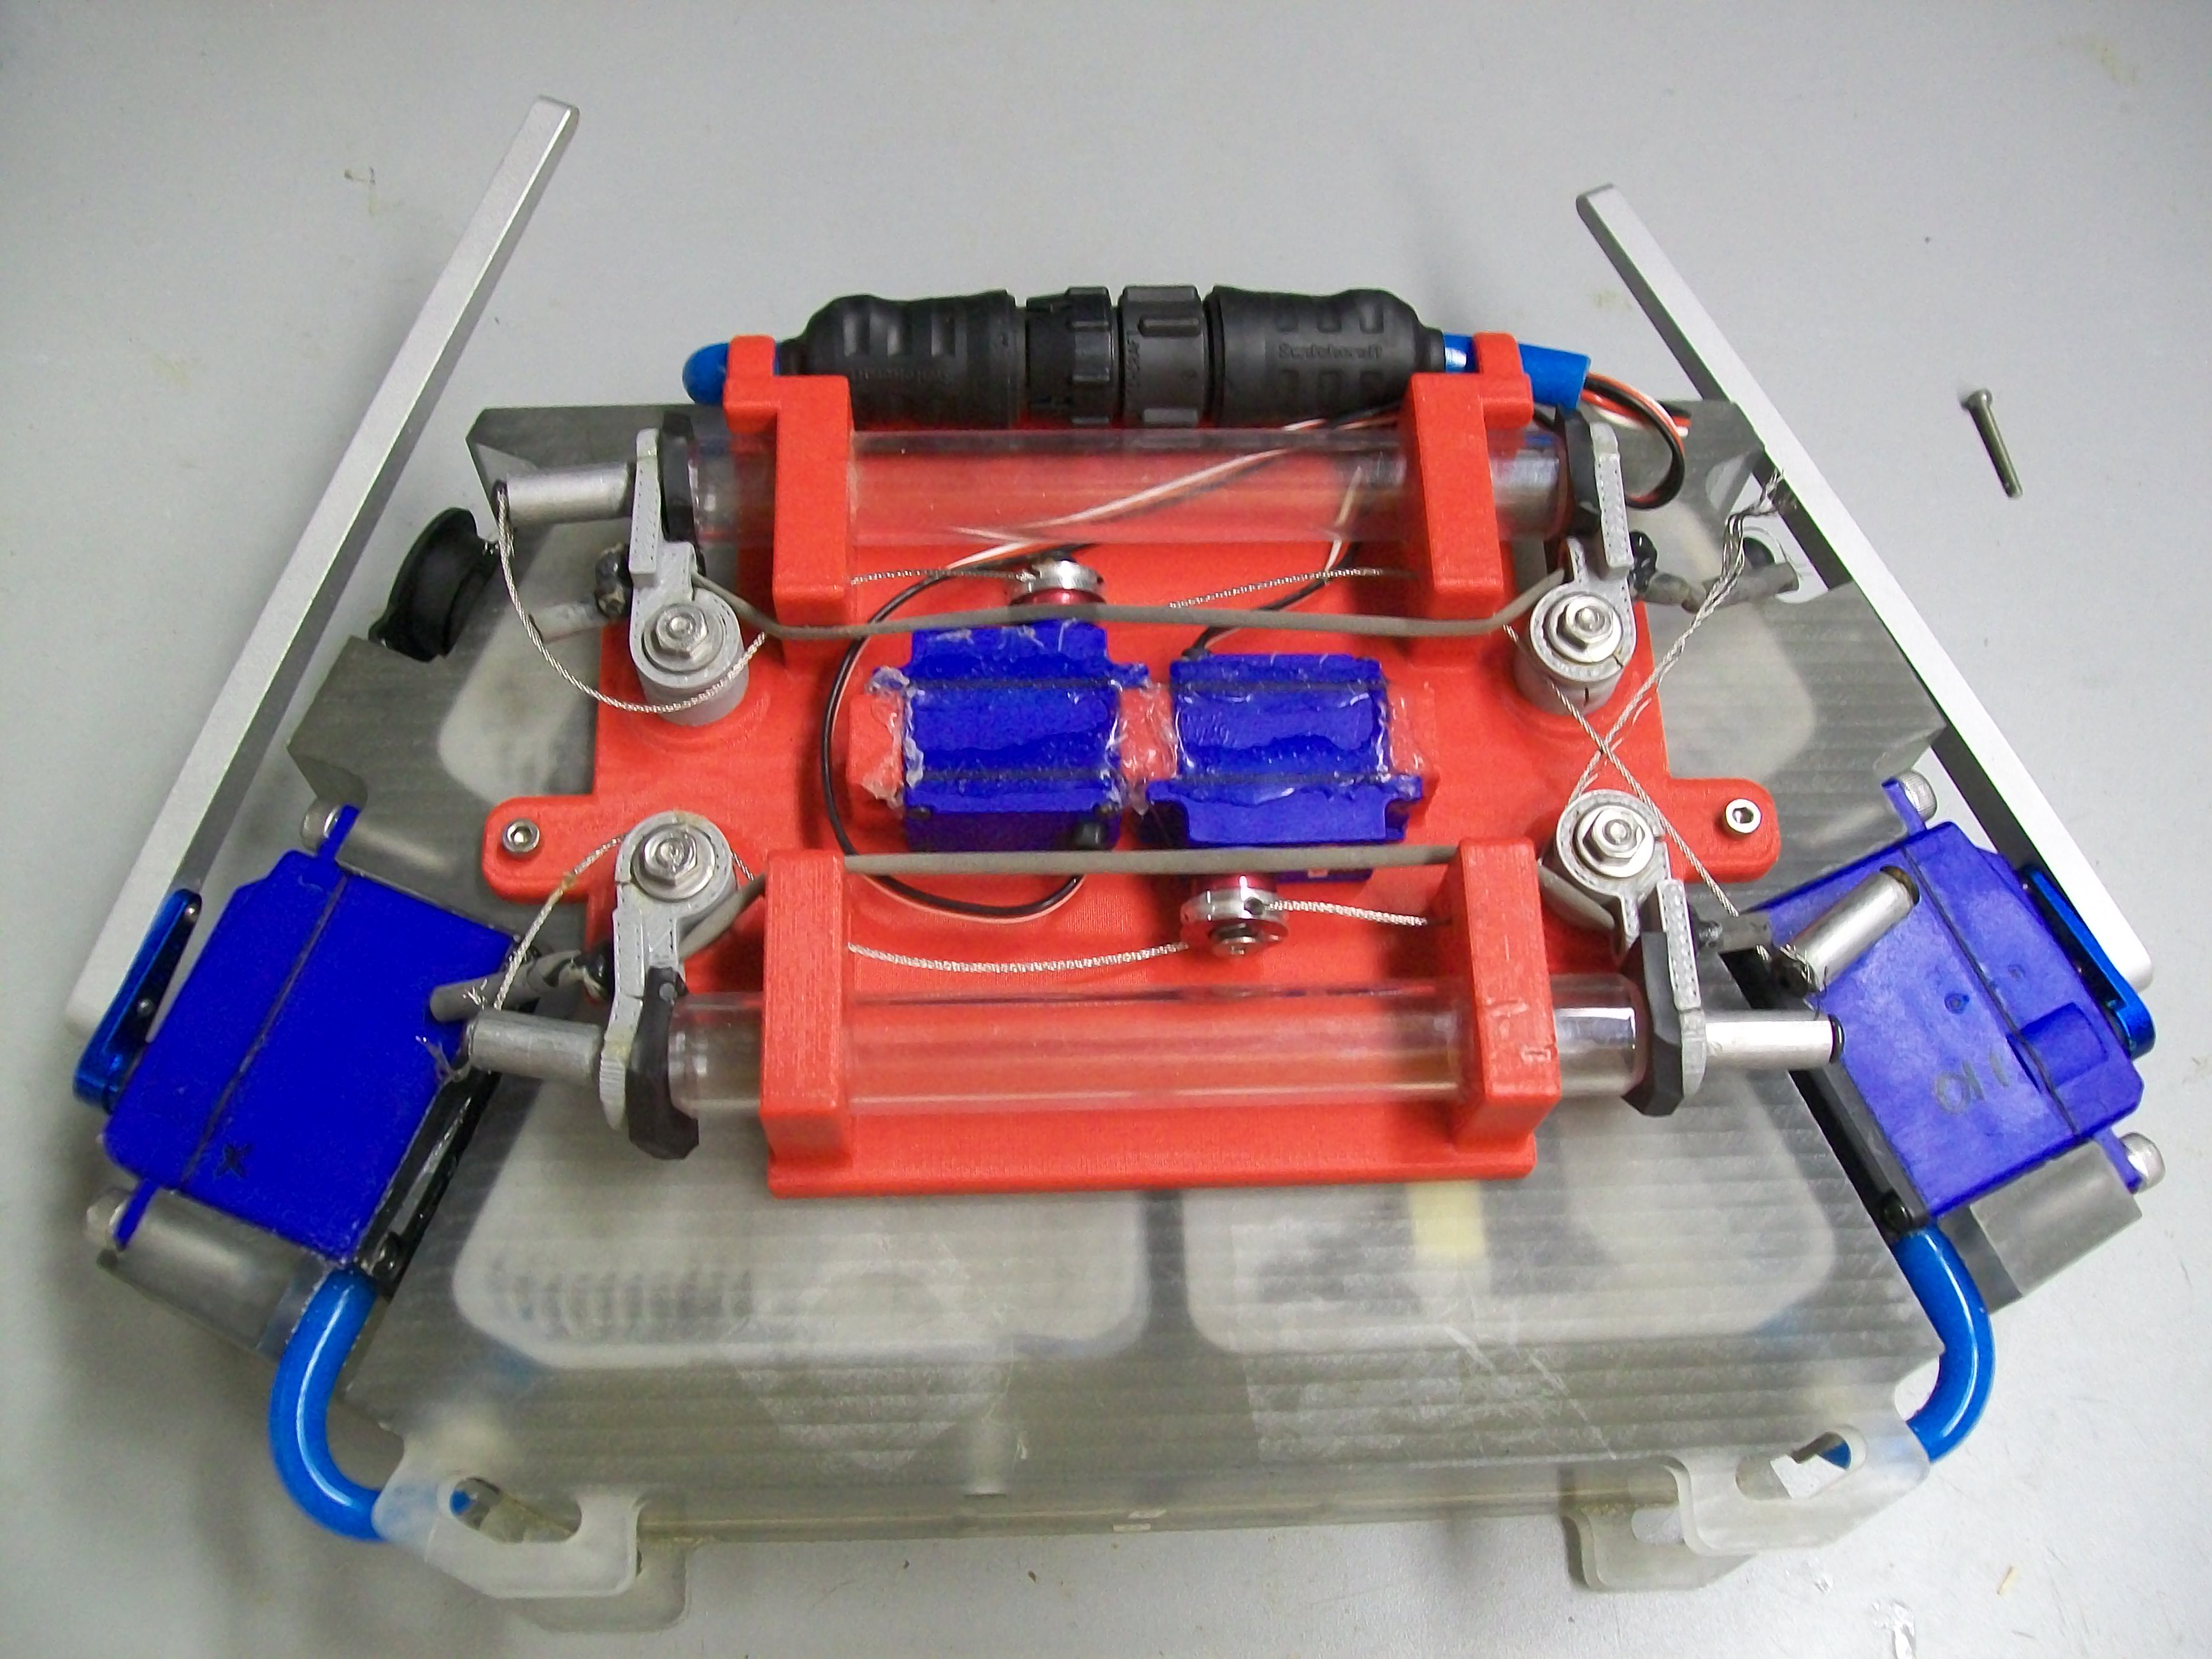
\includegraphics[width=1\columnwidth]{images/sampler.jpg}
  %photo from diving well day
  \caption{Aquapod with attached fluidic sampler suite}
\label{fig:aquapod-and-sampler} \end{figure}

Environmental monitoring is a key area ripe for automation via the use of
robotic platforms. Fluid samplers are often used for limnographic studies, such
as in the work of Villar-Argaiz et al. \cite{Villar-Argaiz2001} where monitoring
the amount of phosphorous and nitrogen compounds was needed to determine factors
that affected the growth of phytoplankton in these lakes.

This type of sampling proves to be very resource intensive as they have to be
done under human supervision. Furthermore, there can be additional costs for
transportation, preparation, and deployment. All of which contribute to the
inertial costs associated with data gathering and can contribute greatly to the
quantity and quality of the data that is produced. Cases like these would
benefit greatly from the automation of data collection, as is available through
autonomous robotic platforms, such as the Aquapod.

The sampler module developed for the Aquapod is of the Van Dorn design
\cite{Robertson1968}, \cite{Villar-Argaiz2001}, \cite{Biggs2012}.   It adds the
ability to take uncontaminated fluid samples and carry them to the surface,
where they can be extracted and properly stored for posterior analysis in a
proper lab environment. Figure \ref{fig:sampler_callout} shows the underside of the
Aquapod with the sampler attached.  The sampler module consists first of two
clear plastic tubes held in place with both ends open.

Swiveling caps, also mounted on the same object holding in the tubes, can seal
off each end of the vials, with rubber adhered to the ends to give a more
effective seal.  The ends are held passively up against the ends of the vial by
a rubber cord stretched between the two caps.  Finally, the caps can be pulled
away from the vials by wires attached to a waterproof servo with a pulley in the
center of the module.  The design of the Van Dorn type sampler precludes
ingression of unwanted fluid into the sampling volume due to the
"normally-closed" configuration of the mechanism. Furthermore, sampling is
available from a number of orientations and conditions given the seals at either
end of the fluid vials.

Finally, the power and signal buses are routed through a IP68 Switchcraft
connection to ensure water does not ingress into the robot.  The circuitry
inside the Aquapod is in charge of running the state machine as well as sending
the appropriate signal to open the vials and take samples. The individually
actuated Van Dorn vials allow sampling at separate depth, thus improving the
utility of the sensor suite.

%Each servo’s static seams are sealed against water entry, and an additional
%o-ring is put on the shaft and the circuitry filled with epoxy to protect
%against higher pressure underwater environments.  Each of the two vials can be
%activated independently, pulling the caps back to allow water to enter the
%vials at the specified moment while allowing air to simultaneously escape.
%This method needs no energy to keep the vials shut, relying on the stored
%energy of the rubber cord to keep the vials sealed and only requiring energy to
%open them.  The module is attached mechanically to the Aquapod itself by four
%small screws and corresponding threaded holes in the outside of the Aquapod
%shell.  A waterproof connector and tubing carrying wires provides the power and
%signal for the servos of the sampling module from the power and circuitry
%inside the Aquapod.  The connectors, in addition to being IP68 certified, are
%filled with epoxy to further seal the electrical connections from the
%underwater enviroment.



\begin{figure}[!ht]
  \centering
  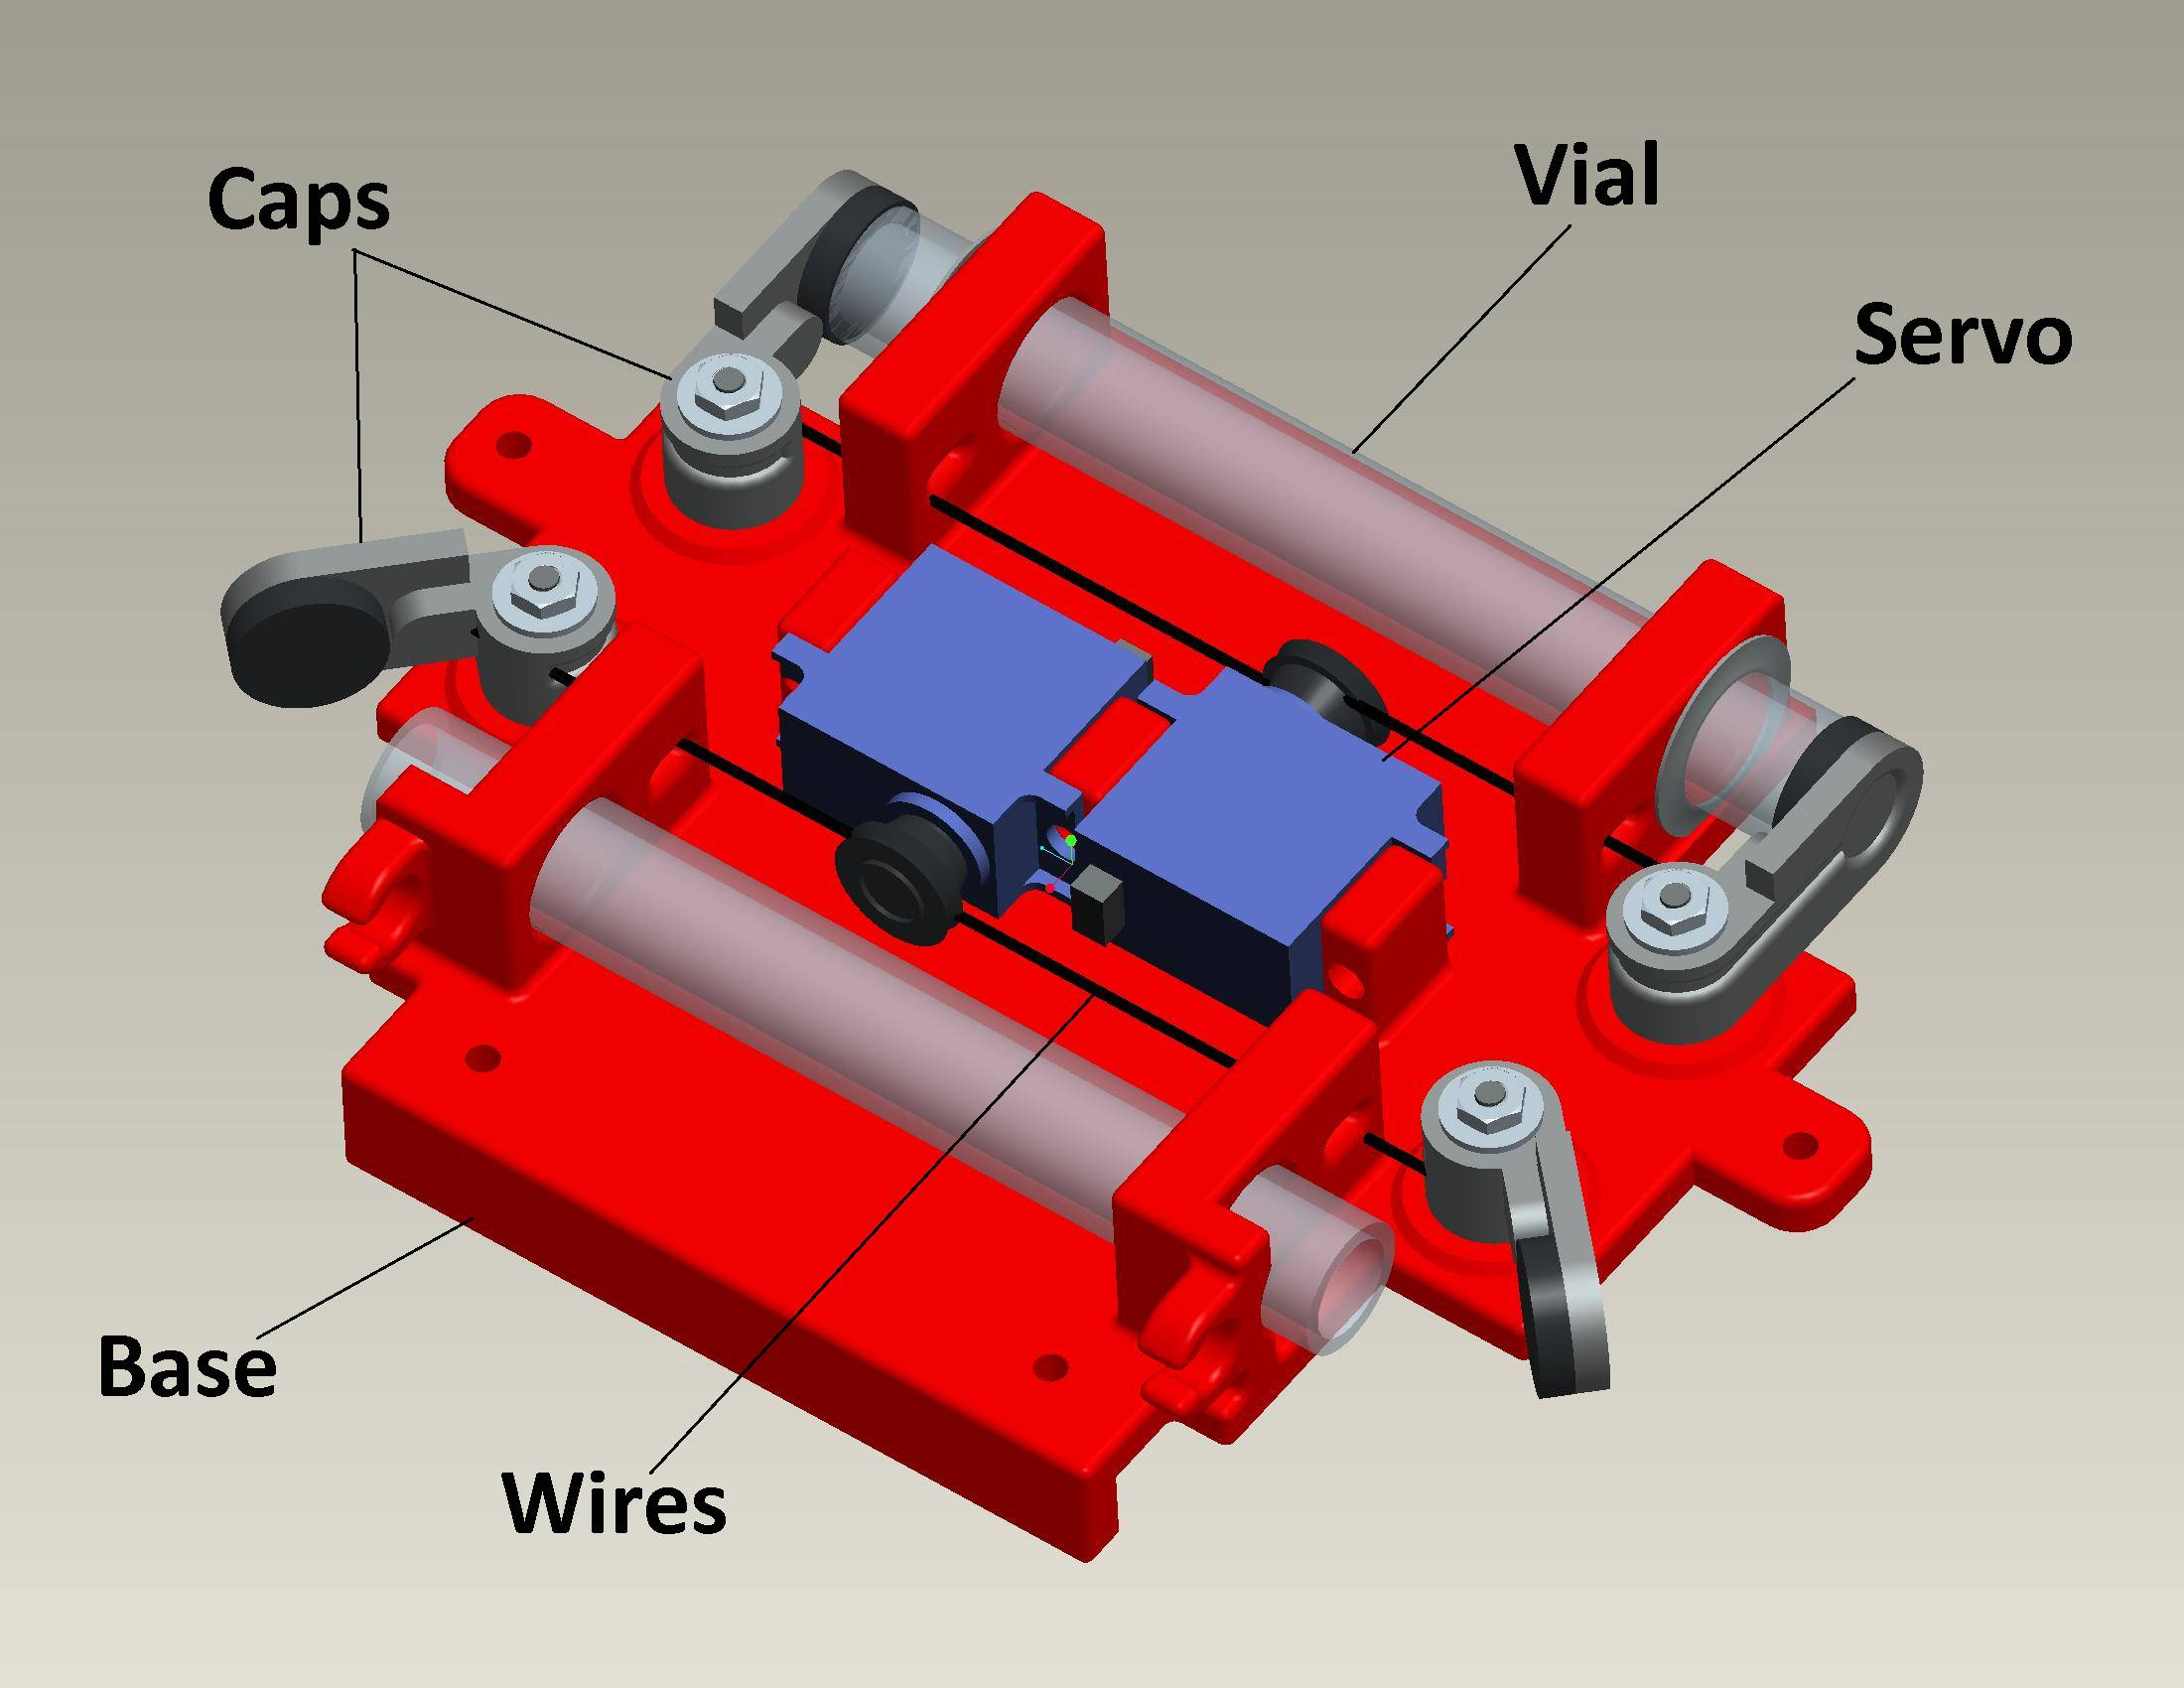
\includegraphics[width=1\columnwidth]{images/sampler_callout.jpg}
  \caption{Annotated fluidic sampler suite}
  \label{fig:sampler_callout}
\end{figure}


% field sampling ...

% Biggs2012, San Diego Bay mercury measurements in marinas.

% Other areas areas are littoral and riverine areas.

% Ref: The horizontal water flow through is not hindered by constrictions so
% that no appreciable contamination can occur in shallow water. As a result, the
% sampler is also suitable for measuring parameters in water with solid
% particles or constituents bound to them, possibly in large quantities.

% Features: minimal contamination since the fluid does not come in contact with
% metallic pieces. Only in contact with the vial material and the lid material.
% Capable of sampling fluids with high concentrations of very large
% particulates. The only limitation is either "mouth" of the bottle.

% Talk about the design of the sampler itself, how it works, why it works - rat
% spring, dropping vials. Talk about the simplicity of the design. Light weight,
% low energy due to normally-closed actuate to open architecture. Fluid
% Flow-through design. Hot-plug type of device. Compact design, mostly flat
% footprint. "Double releaser". The sampler is airtight and as such allows it to
% start in vacuum or from atmospheric air, without intaking fluid on its way to
% the target sampling location and possibly contaminating the vial within. Opens
% at the time of sample, releasing the internal air, and taking fluid only at
% the desired location. Capable of collecting fluid in almost any configuration
% due to the design of the enclosure (structure, exoskeleton, ??) and the
% dual-releaser structure.

% One major added feature to the new Aquapod is the ability to take and hold
% water samples and bring them to the surface for further study external to the
% robot.  With this objective in mind, the sampler module was designed and
% created for the Aquapod.  \figure shows the underside of the Aquapod with the
% sampler attached.  The sampler module consists first of two clear plastic
% tubes held in place with both ends open.  Swiveling caps, also mounted on the
% same object holding in the tubes, can seal off each end of the vials, with
% rubber adhered to the ends to give a more effective seal.  The ends are held
% passively up against the ends of the vial by a rubber cord stretched between
% the two caps.  Finally, the caps can be pulled away from the vials by wires
% attached to a waterproof servo with a pulley in the center of the module.
% Each servo’s static seams are sealed against water entry, and an additional
% o-ring is put on the shaft and the circuitry filled with epoxy to protect
% against higher pressure underwater environments.  Each of the two vials can be
% activated independently, pulling the caps back to allow water to enter the
% vials at the specified moment while allowing air to simultaneously escape.
% This method needs no energy to keep the vials shut, relying on the stored
% energy of the rubber cord to keep the vials sealed and only requiring energy
% to open them.  The module is attached mechanically to the Aquapod itself by
% four small screws and corresponding threaded holes in the outside of the
% Aquapod shell.  A waterproof connector and tubing carrying wires provides the
% power and signal for the servos of the sampling module from the power and
% circuitry inside the Aquapod.  The connectors, in addition to being IP68
% certified, are filled with epoxy to further seal the electrical connections
% from the underwater enviroment.

%The sampler module was designed and created for the Aquapod in order to capture
%water samples and bring them to the surface. Equipment utilized to carry out
%substance detection methods are not practical in miniature robots, therefore,
%collecting these samples is valuable. Furthermore, a more thorough analysis of
%the samples can be done in a laboratory setting.

%Figure \ref{fig:sampler} shows a rendering of the sampler module which attaches
%to the backside of the Aquapod. The module is designed with energy efficiency
%in mind to prolong battery life: thus, two caps on each end of a tube are held
%closed by an elastic band requiring no electric power to remain closed. A servo
%is engaged only to open each end and take the sample, then released to close
%the vials again. The caps are padded with a rubber surface, while the tubes
%have been filed to a sharper end to promote higher pressure between the tube
%and the caps (by reducing the contact area) and thus more effectively sealing
%the vial.

%The current model has two vials, each opened by its own servomotor. The motors
%themselves required additional modifications to survive the maximum design
%pressure: marine sealant was applied to each seam in the plastic body, a
%thicker O-ring was placed on the shaft of the servo to seal it, and the
%circuitry inside the servo was covered in epoxy. This extended the life and
%longevity of these servos to withstand pressures at 10 meters of depth for the
%duration of testing. A waterproof connector runs into the hull of the Aquapod
%to connect power and signal lines to the interior electronics. These connectors
%are also injected with epoxy to ensure a waterproof connection. The backpack
%itself is attached to the Aquapod hull using screws for easy removal.




\subsection*{Screwdrives}

\section*{Proposed Research}

Using identification techniques  



\section*{Preliminary Results}

The tumbling mode of locomotion presents a great advantage in a marked increase
in terrainability with respect to other methods of locomotion employing a
similar size and complexity. That said, motion planning and control in general
are very complex for this mode \cite{Hemes2011}.

The Aquapod can use its BCU to control its vertical ascension and descension
rates, however, it does not have control authority once its arms are not within
reach of a hard surface to push against, such as when in suspension in a column
of fluid or on the bottom of a lake or pool. In these scenarios control is
difficult to achieve, due to the aforementioned inherent difficulties of
tumbling locomotion. These difficulties are magnified by an decrease in apparent
weight of the robot when in water.

The current undertaking in the use of alternative modes of locomotion in
addition to tumbling with the arms in order to facilitate actuation, control,
and planning while still preserving the great mobility provided by tumbling
locomotion.



\subsection{Screwdrive}

A novel type of propulsion is proposed that would allow programmable and precise
movement both on land and water. This modality of locomotion is referred to as a
screwdrive locomotion. Screwdrives are not currently utilized for vehicular
transport and much less in robotics, instead it finds a place in the
manufacturing industry for precise conversion of rotational to linear motion in
applications such as conveyor belts.


The screwdrive will consist of two independently actuated continuous propellers.
On land these can be actuated independently in a manner similar to tank treads
or omnidirectional wheels, however, since the arms retain their capability of
rotation, they will also allow tumbling locomotion for terrainability purposes .

In water, the screwdrives act as continuous propellers. This form of actuation
can be employed both on the surface and while suspended. The rotation of the
screwdrives allows vectoring of the propulsion in such a manner as to increase
the controllability of the robot.

Screwdrive propulsion is a relatively unused method of locomotion that has been
shown to successfully propel military, scientific, and recreational vehicles
across a wide variety of terrains ranging from snow to water and mud to sand
\cite{Fales1972, Cole1961c, Dugoff1967}. Most of this research dates back to the
1960s and 1970s.



Even though the Aquapod has great terrainability on
land \cite{Hemes2012} on land, it is severely limited in the water. Attempts
have been made to integrate flipper-like appendages to the existing arms,
however, the torque and speed requirements for \emph{swimming} with the flippers
are not compatible with those necessary for \emph{tumbling} on land.


There are a number of applications for which an amphibious robot would need
precise control of its attitude underwater. The Aquapod as a mobile robotic
platform does not have the capacity in energy, speed, power, or advanced
electronics to perform complex tasks itself and maintain the flexibility
required of an amphibious robot. Due to its multiple theaters of operation,
modularity affords the robot an amount of flexibility that enables it to
accomplish a number of tasks that is much greater than if one robot was designed
to accomplish all these tasks by itself.

One advantage of pursuing small robot applications is the capability of
producing many small robots that can work together with a differentiated sensor
suite to accomplish a goal, as a team, that could not be realized individually.
One can imagine a situation where one of these small robots can have advanced
sensors to detect the presence of unknown objects in a body of water while
underwater, while another Aquapod on the surface, has an advanced communications
suite that allows it to communicate with the underwater members of the team and
with a on-shore command center via telecommunications.  Given that this small
robot's greatest strength lies in its abilities to operate in amphibious
environments, it is an understatement to say that there is a need to provide a
means of locomotion for the robot that maintains its small size, simplicity, and
relatively low price. Furthermore, assuming that a suitable propulsion method is
found, the problem of attitude control while in the three-dimensional space that
is open water remains.

One promising research direction is utilizing a, now, unusual form of locomotion
that employs screws with relatively high blade height to provide propulsion as
the screw turns in the water. In effect, it is analogous to a submersed
Archimedes screw \cite{Freeberg2010} or a long and continuous
propeller\cite{Cole1961c}.


Currently, the robot does not have a level heading when in the water. Due to the
space-allocation constraints in the limited internal space of the Aquapod, the
robot sits off kilter when in water in the roll and pitch axes. With one buoyant
tip, depending on which arm it’s placed on, the robot would be able to alter its
pitch, but would introduce some unwanted change in the roll axis. With two
buoyant tips, both axes could be affected such that a determined attitude can be
achieved. Controlling the pitch and roll of the robot would also allow for
controlled gliding situations, where an optimized exterior hull, and the
buoyancy control unit can be used to provide energy efficient gliding.

As can be seen in \ref{fig:aquapod_v1_pool} the arms are at an angle to the
saggital plane of the robot. This fact can allow asymmetrical application of the
buoyancy forces of the arms to provide roll control as well as pitch control.
Where roll control is rotation about the longitudinal axis \emph{x}, pitch is
rotation about the axis \emph{y}, and yaw is rotation about the \emph{z} axis.
See figure \ref{fig:auv}. This mechanism would be analogous to that studied by
\cite{Libby2012}, where lizards' use of their tail to control their pitch was
studied with a robotic prototype.

\begin{figure}[tb] 
\centering
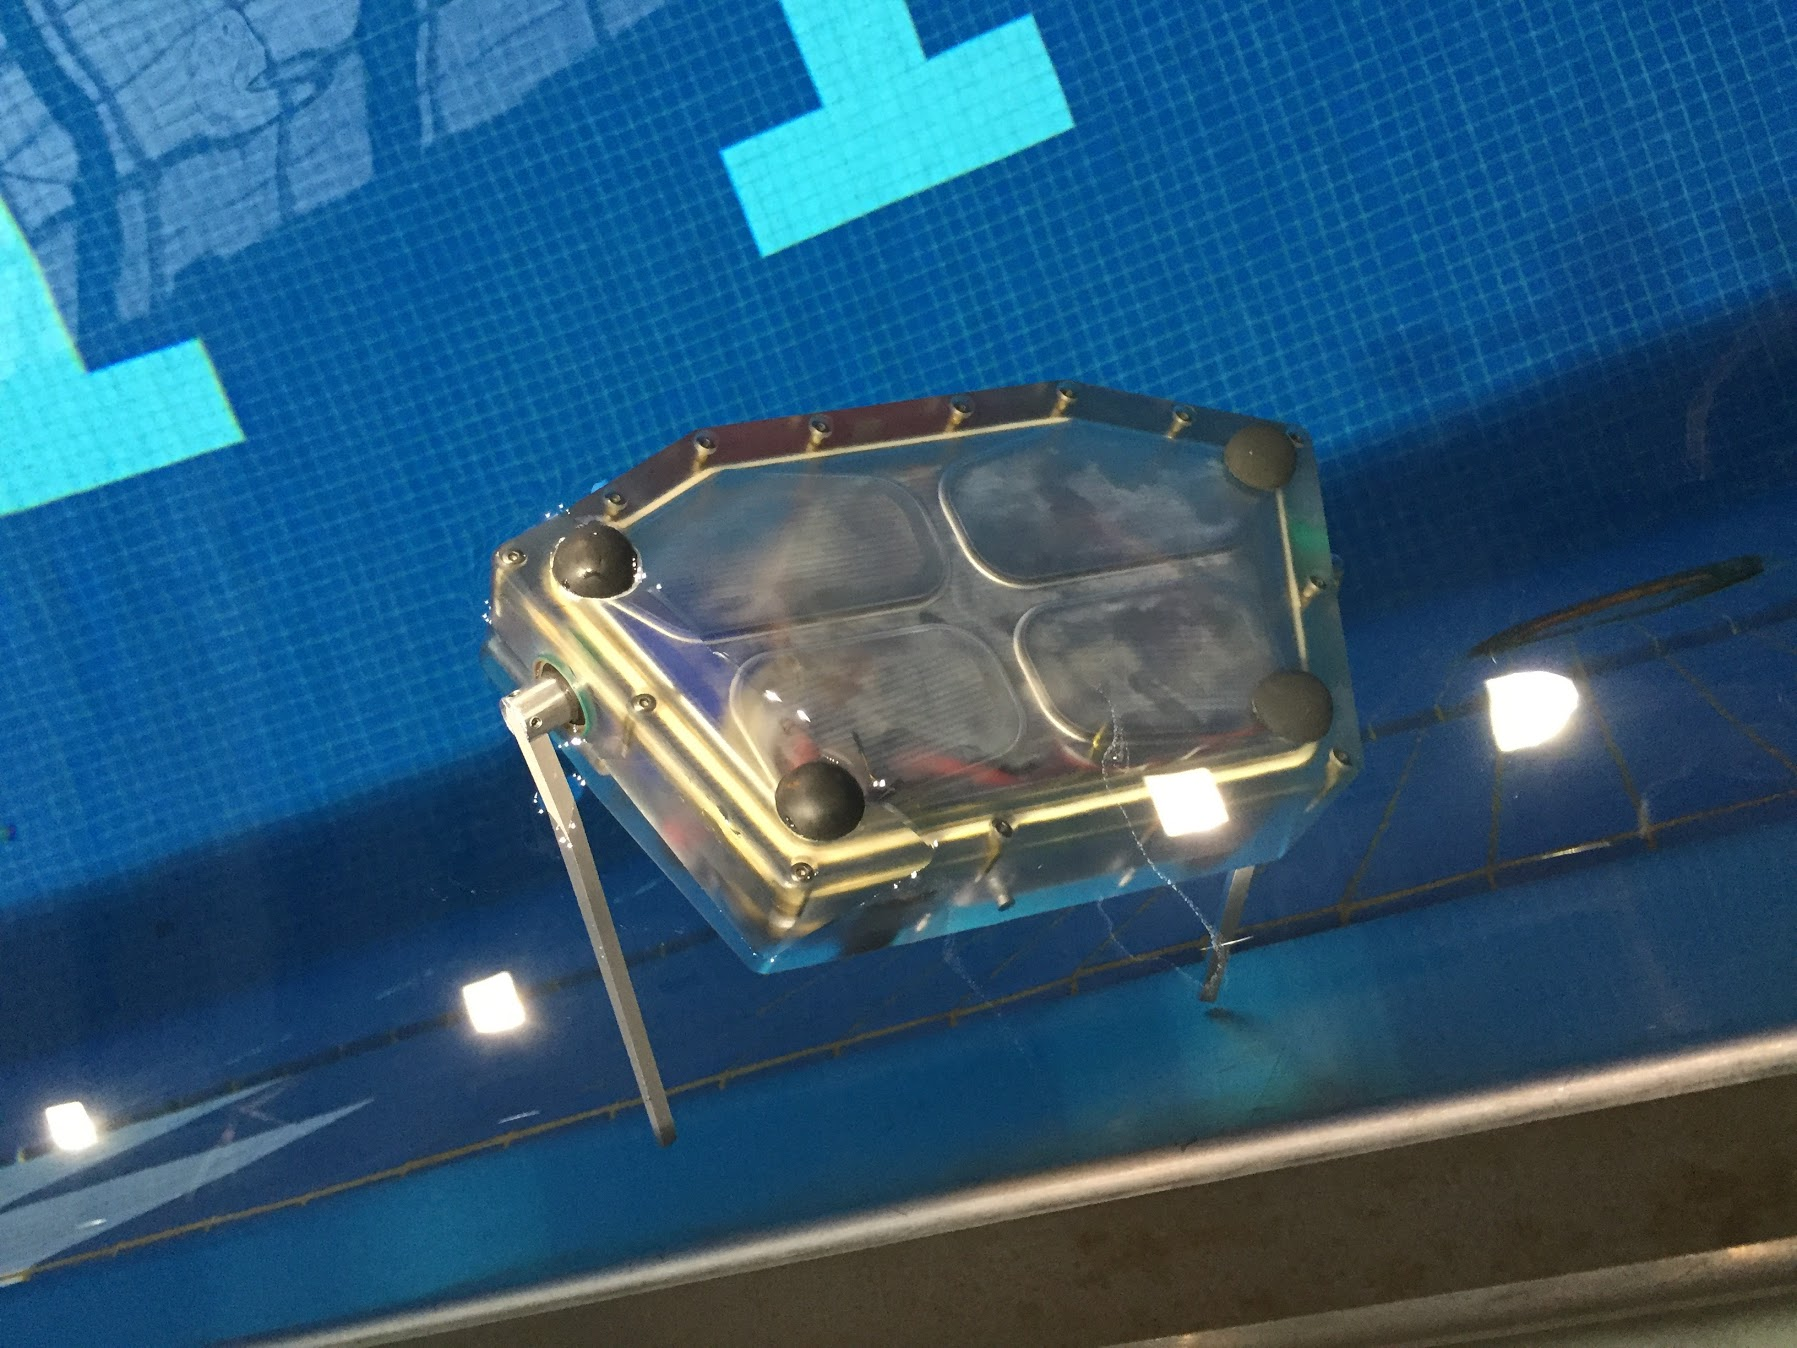
\includegraphics[width=1\columnwidth]{images/aquapod_diving_well.jpg} 
%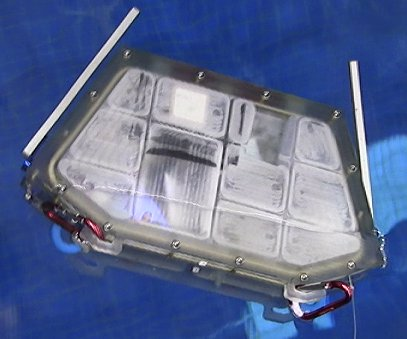
\includegraphics[width=1\columnwidth]{images/aquapod_v1_pool.jpg} 
\vspace{-10pt}
\caption{Aquapod}  
\vspace{-20pt} 
\label{fig:aquapod_v1_pool} 
\end{figure}

% #TODO check what image aquapod_v1_pool referred to in the original paper 


\begin{figure}[tb] 
\centering
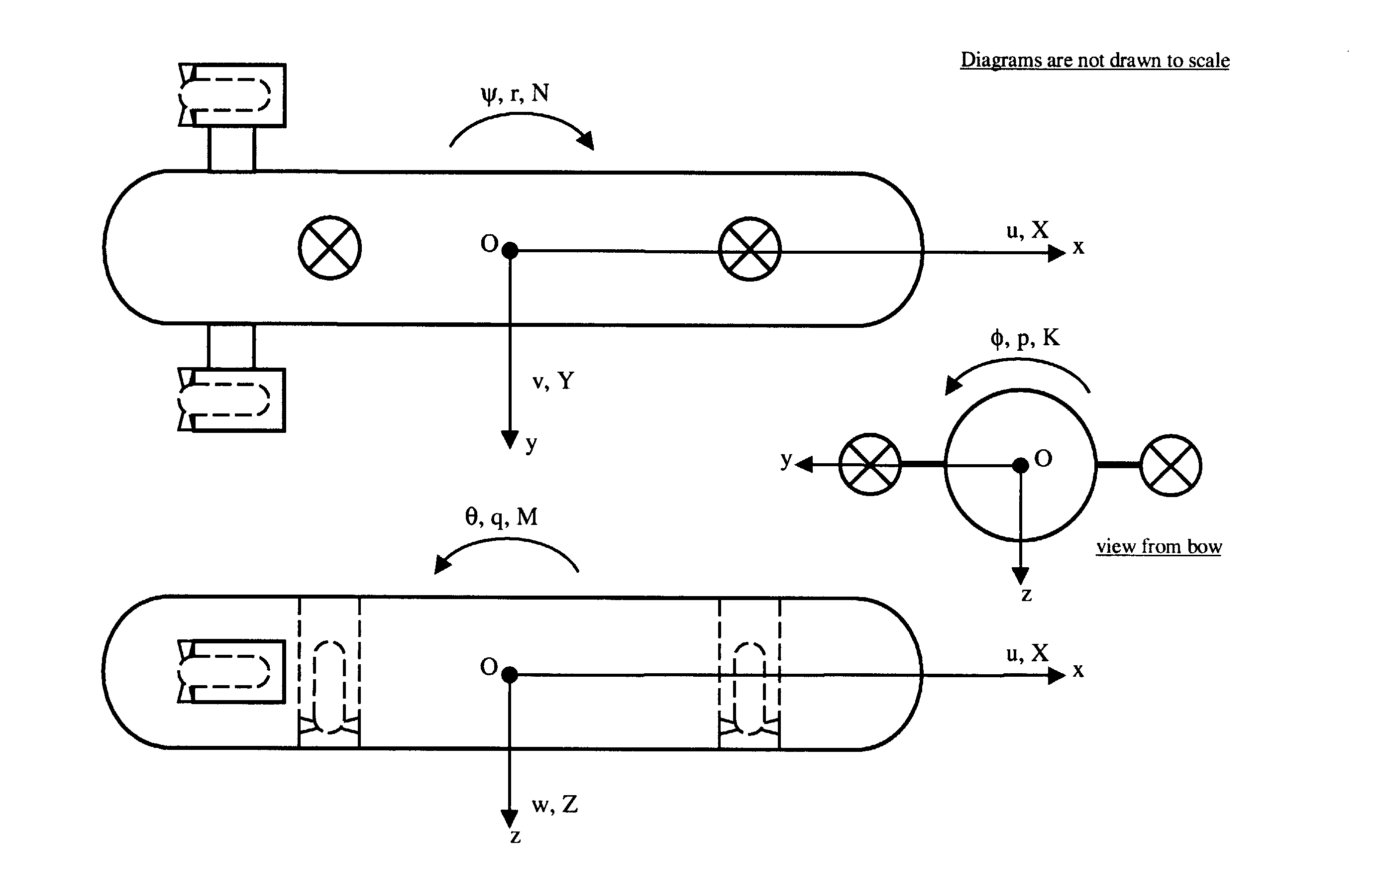
\includegraphics[width=1\columnwidth]{images/auv.jpg} 
\vspace{-10pt}
\caption{AUV used in simulation and axes representation}  
\vspace{-20pt}
\label{fig:auv} 
\end{figure}

It is necessary to simulate the behavior of any design change in order to study
the feasibility and, possibly, optimize the design of a potential prototype. The objective is to find a suitable set of equations of motion and hydrodynamic
force and moments description such that system identification methods used for
UAVs could be applied in the future \cite{Dorobantu2011}.

Due to the non-linear of the fluid dynamics and the difficulty of empirically
determining the hydrodynamic coefficients. There seems to be two main ways of
simulating and solving the 6DOF equations of motions for a submersed vehicle.
One way involves simplifying the equations of motions and having a very high
fidelity model, such as \cite{Humphreys1981}. The other approach takes the
opposite path and simplifies the hydrodynamic coefficients to the point where
they can be calculated based off typical structures (such as cylinder shaped
AUVs), but using the non-linear form of the equations of motion \cite{Nahon}.

The approach taken by \cite{Tang1999}, retains the non-linear rigid body
dynamics as Nahon, however the hydrodynamic forces and moments are described as
in \cite{Fossen2011}, where the hydrodynamical model consists of all the forces
and moments acting on the body. These forces and moments are decomposed into
radiation-induced, environmental and propulsive forces. This is at the same time
less empirical than Humphreys \cite{Humphreys1981} which relys solely on
empirical results to determine said forces and moments.

\subsubsection{Methodology}

The long term methodology is to identify a suitable framework that will allow
simulation of buoyant and propulsive arms. This method should allow for
posterior analysis and identification of a higher fidelity system model.

The short term methodology is to use the existing frameworks for simulation of
dynamical maritime vehicles. Due to the cost in time and instrumentation
necessary to determine all the relevant coefficients that describe the sum of
the forces and moments acting on a body in the water, it is desirable to find a
sample AUV to serve as a data set from which to part for posterior modification
to fit the Aquapod.

The Autolycus was chosen as the sample AUV since the framework model described
by Tang and Leonard \cite{Tang1999} had a great balance of model fidelity, due
to keeping the nonlinear terms of the equations of motion, yet was feasible to
model without stringent empirical calculation of the hydrodynamic properties of
the AUV.

The combination of the non-linear rigid body dynamics and the use of all the
moments and forces acting on the AUV should allow an accurate model without the
need to spend a excessive use of resources to empirically determine all they
hydrodynamic forces and moments. The model used by Tang \cite{Tang1999}
maintains the non-linear behavior of the AUV. The hydrodynamic effects acting on
the vehicle are modeled as components of the added mass, viscous damping,
restoring and propulsion forces and moments. Furthermore, this relatively simple
model is simple to describe and comprehend theoretically.

Furthermore, using Tang's model allows us to effectively model the Aquapod, once
the relevant hydrodynamic properties have been determined empirically, in
three-dimensional space.




\subsection{Screwdrive Blade Forces}

Two independent screw-like actuators rotate to propel the vehicle forward,
backward, laterally, and to allow rotations in place, see Figure~
\ref{fig:screw_FBD_alpha_0}. The screws consists of an cylinder with wrapped
helices. When rotated in a coordinated fashion, these allow the variety of
movements mentioned above.

There is a difference in available mobility profiles depending on the type of
terrain, that is, in water and soft terrains the screwdrive will function
differently than on hard terrains. This is due to the ability, or lack thereof,
of material penetration by the helix blades. On soft terrains the screws cut
into and displace material entrained between its helices once actuated. On hard
terrains, the helices are not able to dig in and exhibit a different mobility
profile.

This dependency on the hardness of the terrain manifests itself most prominently
when trying to more forward or backward on hard terrains and on the ability to
rotate in place in soft terrains and opposed to the lateral movements available
on hard terrain.

This duality of movement profiles presents interesting challenges from the
system modeling and control perspective. One objective is to build, design, and
test a system model and relevant controller a to allow path planning.

%the compensation for desirable movements that may be required during the course
%of a mission.One  alternative  to  be  studied  is  the  use  of  an  extra
%screw  to  provide  extra  controllability,  another  is  to incorporate a
%rotating body design.  Rotating the body will allow using the available
%mobility directions tomove throughout the environment while rotating the
%sensors.


\subsection{Screwdrive forces}

The screws provide a combination of tractive and rolling forces. The tractive
forces are those created from the longitudinal displacement of material against
the screw's helix. The rolling forces are the ones that result from the rotation
of the cylinder about its axes. In Figure~ \ref{fig:screw_FBD_alpha_0} two
contra-rotating screws are shown.

\emph{Rolling forces} are akin to those of the wheels on a vehicle. The wheels
turn and, given enough friction with the surface it is rolling on, push the
surface to provide movement in the same direction as the wheels are turning.

\emph{Traction forces} as they have been called in \cite{Freeberg2010}, result
from the blade of the screw digging into and pushing against material. In the
case that the material is a solid, such as dirt or snow, then the screw propels
itself forward in a manner similar to the \emph{rolling force} modality. On the
other hand, if the material is a fluid, such as water, then the screw pushes the
fluid in a direction and creates \emph{thrust}.

%\section{Rigid versus soft terrains} The problem with the current \emph{double
%screw} setup is that it is not capable of providing full directional control of
%movement.  In water the \emph{double screw} can effectively turn in place and
%move forward or backward, giving it the capacity to move throughout its
%environment.  On land, if the screws cannot dig into the terrain, such as on a
%hard floor, cement, ice, etc, then the forward and backward propulsion due to
%the screw is lost. Furthermore, rotation is not possible with a standard double
%screw setup.  On the other hand, rolling works well and the double screw can
%move laterally.

\subsection{Inter-screw angle}

The inter-screw angle affects the direction in which the tractive and rolling
qorces are exerted. Furthermore, in systems with two independently actuated
screws, the inter-screw angle affects the resulting motions from the net forces
of the competing or cooperating screws. The redirection and interplay of the
forces from the dual-screw set-up can be seen in
Figure~\ref{fig:screw_FBD_alpha_0} and Figure~\ref{fig:screw_FBD_alpha_45} where
the inter-screw angle is set to 0 and 45 degrees, respectively.


\begin{figure}[ht] \centering
\includegraphics[scale=0.25]{images/screw_propulsion_FBD_alpha_0.pdf}
\caption{Inter-screw angle of 0 degrees(parallel)} \label{fig:screw_FBD_alpha_0}
\end{figure}

\begin{figure}[th] \centering
\includegraphics[scale=0.25]{images/screw_propulsion_FBD_alpha_45.pdf}
\caption{Inter-screw angle of 45} \label{fig:screw_FBD_alpha_45} \end{figure}


A change in the inter-screw angle \( \alpha \) will imply a change in the
balance between the rolling and thrust forces. Utilizing \( \alpha \) it is
possible to induce a net longitudinal motion even on rigid terrains. However,
some of this force will be lost to the lateral component. Similarly, on water,
the full force of the thrust will not be used for longitudinal motion as some of
it is lost to equal but opposite lateral trust components that cancel out.

\subsubsection{Vector force analysis for a certain inter-screw angle}

\begin{figure}[th] \centering
\includegraphics[scale=0.25]{images/screw_propulsion_FBD_alpha_45_rigid.pdf}
\caption{Inter-screw angle of 45 on rigid terrain.}
\label{fig:screw_FBD_alpha_45_rigid} \end{figure}


\begin{figure}[th] \centering
\includegraphics[scale=0.25]{images/screw_propulsion_FBD_alpha_45_water.pdf}
\caption{Inter-screw angle of 45 in water (rolling forces are negligible)}
\end{figure}


\begin{figure}[th] \centering
\includegraphics[scale=0.25]{images/FBD-two-screw-45-rigid-rotation.pdf}
\caption{Rotation with an inter-screw angle of 45 on a rigid terrain}
\end{figure}

\begin{figure}[th] \centering
\includegraphics[scale=0.25]{images/FBD-two-screw-45-rotation-water.pdf}
\caption{Inter-screw angle of 45 on a rigid terrain rotation)} \end{figure}



%\section{Solution 2: Screw helix angle}

%Questions \begin{itemize} \item Where does this parameter come from? (The
%optimum is 30 $^\circ$) \item \end{itemize}

%Without knowing the magnitude of the forces generated due to the interaction of
%the screw with the terrain, we can make some theoretical arguments in favor of
%a favorable helix angle for the direction of the forces generated by the screw
%action of the screw drive. It is important to note that the forces generated
%from the screw motion have both a longitudinal and lateral component.
%Additionally, there always exist rolling forces due to the rolling of the
%vehicle.

%[Check Freeberg]



%\section{Solution 3: Quad-screw configuration}

%\section{Future enhancements} Integrating the screw drive elements to the arms
%of the robot will greatly improve the mobility of the robot. On land it will
%provide a more svelte profile that will allow surpassing obstacles of greater
%size. Additionally, placing the screws on the arms will allow the robot to
%traverse either right-side-up or up-side-down.  Furthermore, in water, the arm
%angle with respect to the body would control the thrust vectors from the
%screws, allowing control in the three-dimensional space that is open water.


%\section{some references}

%\cite{Fales1972} \cite{Dugoff1967}

%\section{Images from overleaf}

%\begin{figure} \centering 
\includegraphics[width=0.45\textwidth]{tyco.jpg}
%\caption{\label{fig:tyco} Tyco Twister toy which used a hinged dual screwdrive}
%\end{figure}

%\begin{figure} \centering
%
\includegraphics[width=0.45\textwidth]{quad-water-2.png}
%\caption{\label{fig:quad_water_2} Quad screwdrive vehicle in water
%(\cite{Freeberg2010}).} \end{figure}

%\begin{figure} \centering
%
\includegraphics[width=0.45\textwidth]{quad-water.png}
%\caption{\label{fig:quad_water} Quad screwdrive vehicle on water surface
%(\cite{Freeberg2010}).} \end{figure}









\subsection*{Screwdrive prototype}
\subsection*{Screwdrive shoulder}

\section*{Conclusion}








\section{Unorganized text}


%\subsection{other}

%The proposed approach will consist of the following stages:  design,
%construction of a prototype, and imple-mentation.The design of the screw-drive
%powertrain will consist of the complete design process for the elaboration
%ofthe prototype.  This includes, but is not limited to, the electrical,
%mechanical, and software-related aspectsof the system and experimentation with
%an existing prototype.  The idea is to study the available screwdriveprototype,
%which was purchased, then design and build a smaller version for the Aquapod
%robot.This smaller prototype would be optimized for a combination of hard and
%soft terrains with emphasis onhard smooth surfaces, such as that of an office
%or building floor, and for water, such that the Aquapod gainsa viable method of
%propulsion in the water.  This prototype will be swappable in that it will use
%the existingexpansion port for control and power.Furthermore,  other
%deliverables  will  include  the  design  and  verification  of  a  dynamic
%model  based  onthe proposed prototype design.  Additionally, a controller will
%be built to accommodate the final prototypedesign.The redesign of the Aquapod
%such that its components can be swapped will require rapid manufacturinga
%number of prototype pieces in such a way that any design challenges that arise
%can be quickly compensatedfor with a redesign.  For this task, additive
%manufacturing techniques, such as 3D printing, will be used forquickly and
%economically iterating over design possibilities.Furthermore, since the design
%of a swappable-part Aquapod will require careful fits between the piecesas well
%as  guaranteeing  hermeticity  of  the  components  and  connections, each
%piece  will  be  treated  as  anindividual unit and will be presented as a
%separate deliverable.





%\subsection{Text NRI draft 2017}

%jaqn to build upon the sensing, propulsion, electronics, control, and
%communication components of the UMN’s Aquapod robot (Fig. 5) (Morellas). The
%%Aquapod is a small form-factor amphibious robot that is equipped with a buoyancy
%control unit (BCU) which allows it to alter its density to descend or ascend in
%a fluid column in a controllable manner. The buoyancy control is a static
%alternative to dynamic diving systems used in some submersibles, proving to be
%more energy efficient to control the robot’s depth by only requiring energy to
%change diving characteristics like sinking or floating. This capability,
%combined with proper control surfaces, also allows efficient longitudinal
%movement in a gliding fashion. The robot is capable of descending to depths of
%up-to 10 meters and collect fluid samples throughout said fluid column. Its
%unique form of tumbling locomotion results in a versatile platform that can be
%used in both terrestrial and aquatic environments leveraging its high
%mobility-to-size ratio. A novel type of propulsion is also proposed (for the
%Aquapod and eventually the jellyfish) that would allow programmable and precise
%movement both on land and water.  This modality of locomotion is referred to as
%a screwdrive locomotion. Screwdrives are not currently utilized for vehicular
%transport and much less in robotics, instead it finds a place in the
%manufacturing industry for precise conversion of rotational to linear motion in
%applications such as conveyor belts.
%
%
%
%Figure 5: The Aquapod robot and its sampling package.  /TODO: add images
%
%\begin{figure}[tb]
  %\centering
  %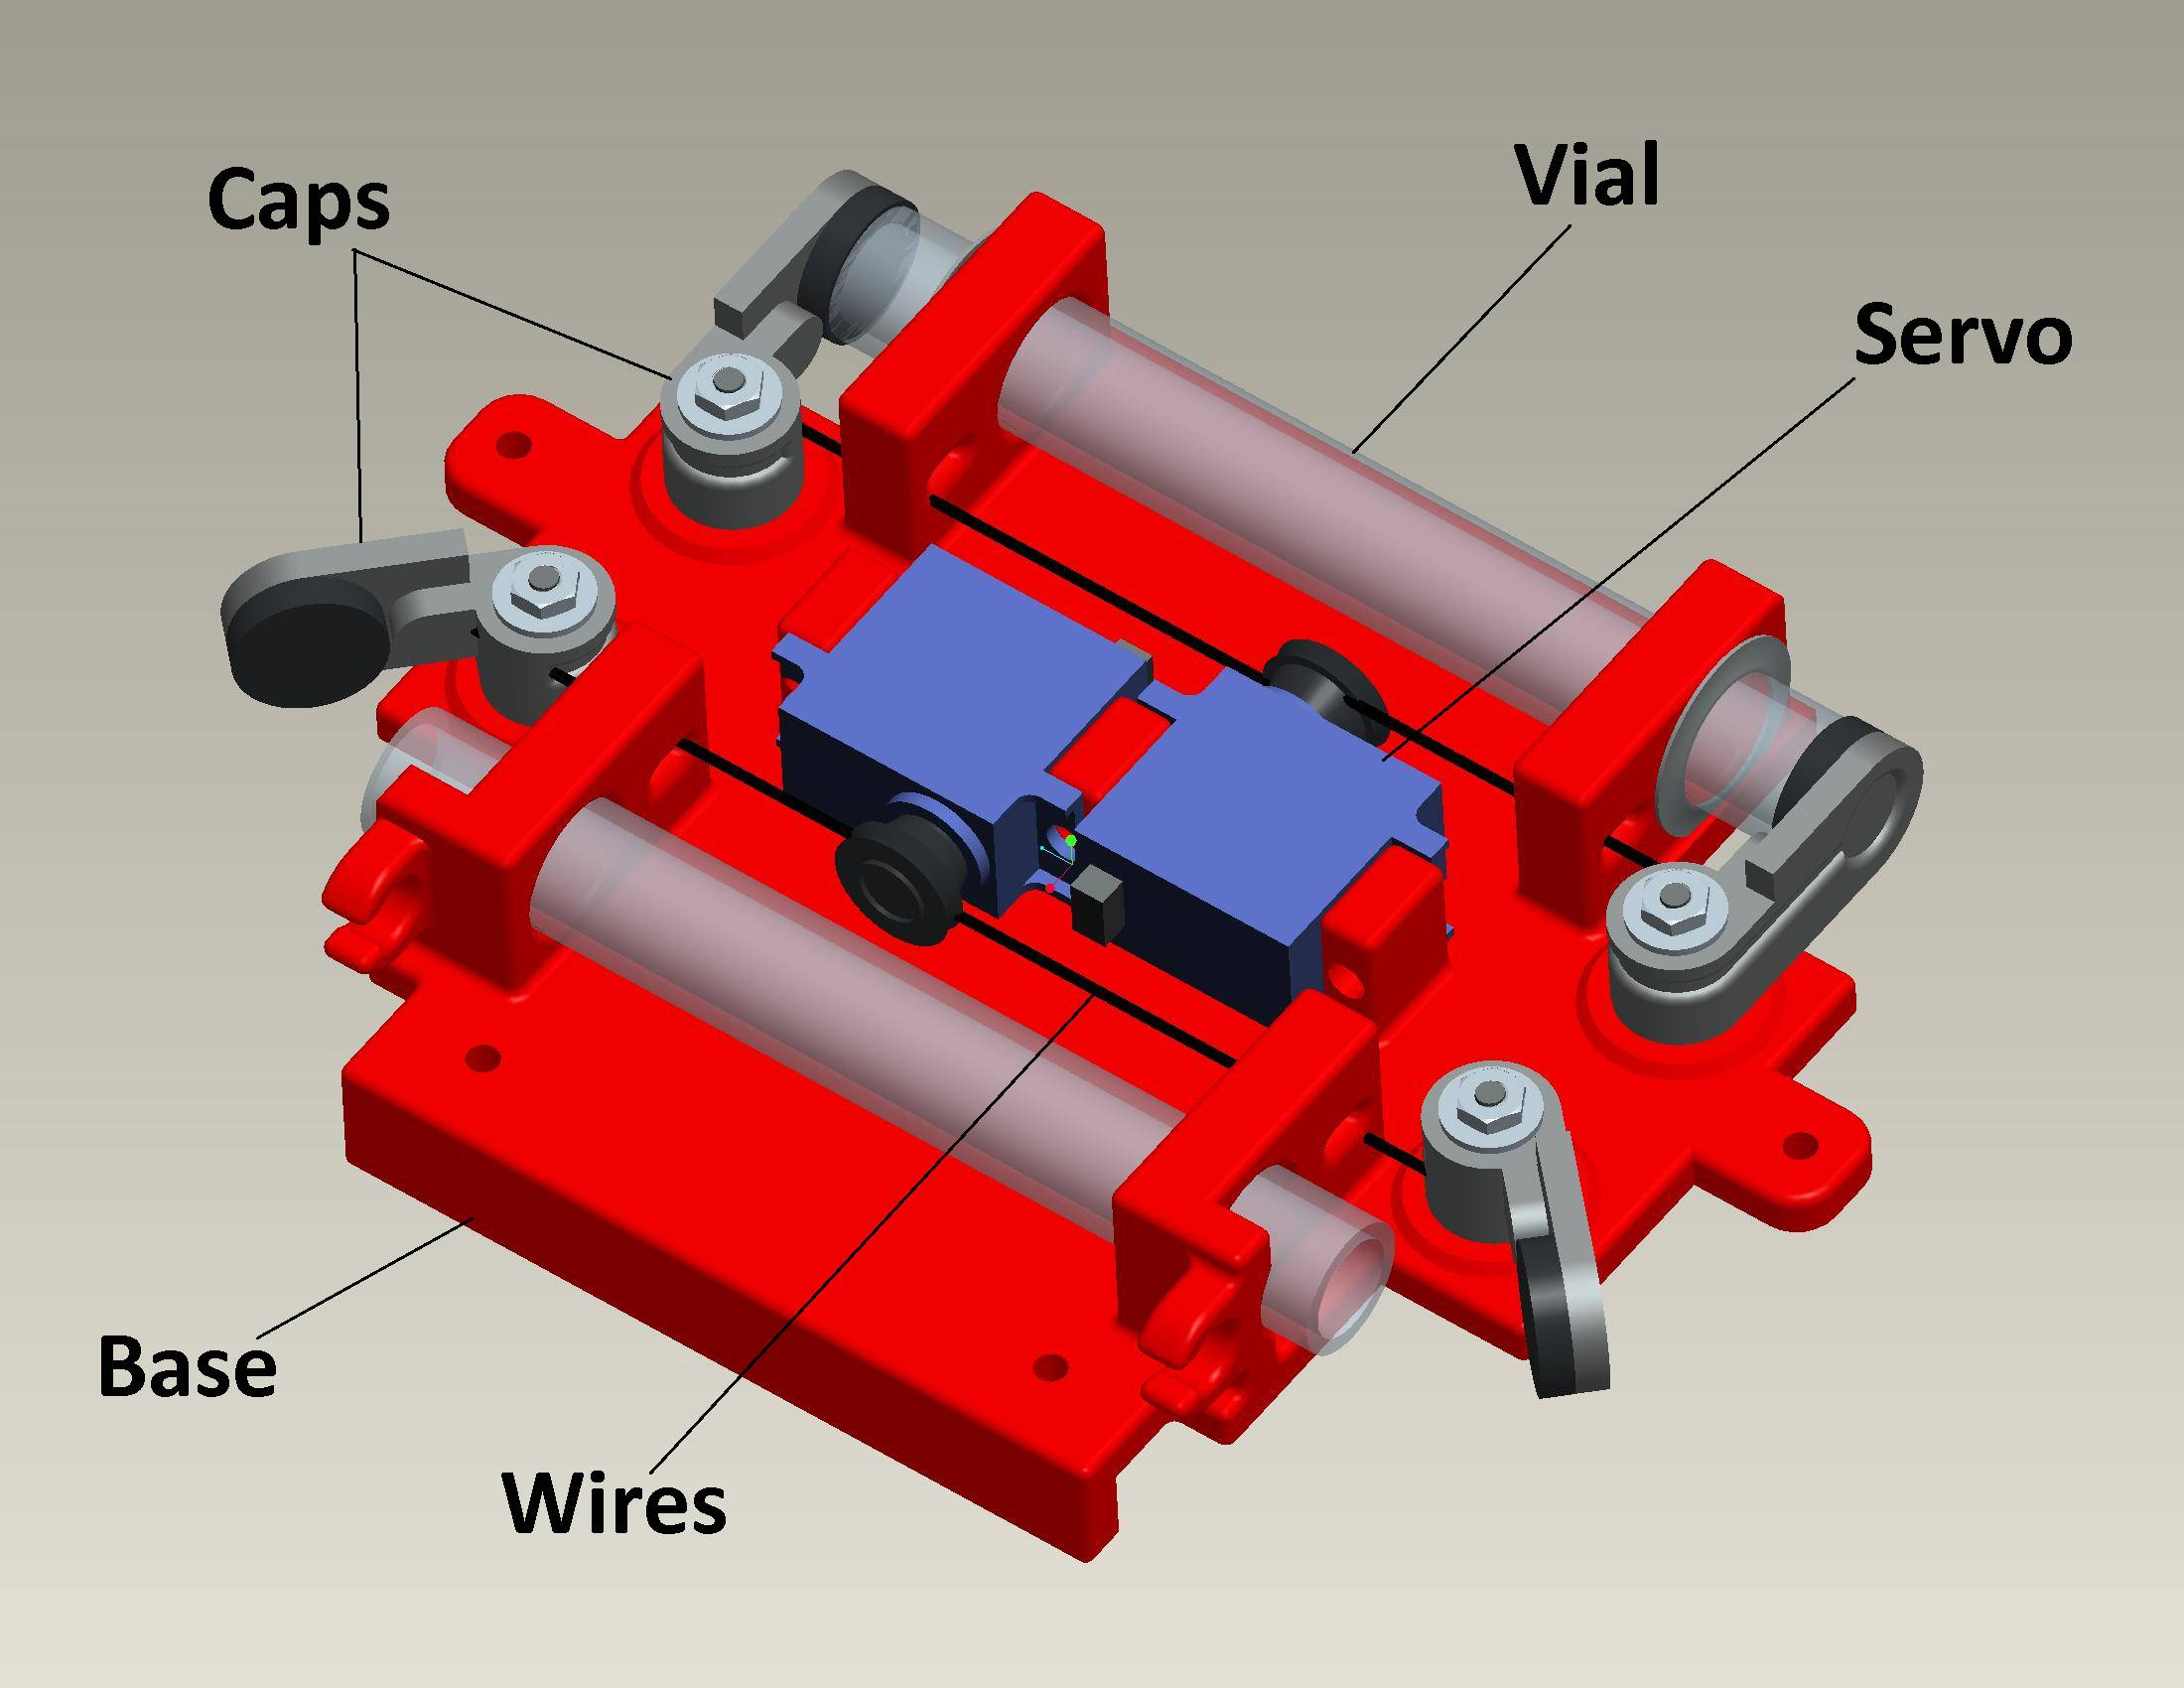
\includegraphics[width=1\columnwidth]{images/sampler_callout.jpg}
  %\vspace{-10pt}
  %\caption{Aquapod}
  %\vspace{-20pt}
  %\label{fig:sampler_callout_nri}
%\end{figure}
%
%
%
%The screwdrive will consist of two independently actuated continuous propellers.
%On land these can be actuated independently in a manner similar to tank treads
%or omnidirectional wheels, however, since the arms retain their capability of
%rotation, they will also allow tumbling locomotion for terrainability purposes.
%In water, the screwdrives act as continuous propellers. This form of actuation
%can be employed both on the surface and while suspended. The rotation of the
%screwdrives allows vectoring of the propulsion in such a manner as to increase
%the controllability of the robot. Screwdrive propulsion is a relatively unused
%method of locomotion that has been shown to successfully propel military,
%scientific, and recreational vehicles across a wide variety of terrains ranging
%from snow to water and mud to sand. Most of this research dates back to the
%1960s and 1970s.
%
%Two independent screw-like actuators will rotate to propel the vehicle forward,
%backward, laterally, and to allow rotations in place. The screws consist of a
%cylinder with wrapped helices. When rotated in a coordinated fashion, these
%allow the variety of movements mentioned above. There is a difference in
%available mobility profiles depending on the type of terrain, that is, in water
%and soft terrains the screwdrive will function differently than on hard
%terrains. This is due to the ability, or lack thereof, of material penetration
%by the helix blades. On soft terrains the screws cut into and displace material
%entrained between its helices once actuated. On hard terrains, the helices are
%not able to dig in and exhibit a different mobility profile. This dependency on
%the hardness of the terrain manifests itself most prominently when trying to
%more forward or backward on hard terrains and on the ability to rotate in place
%in soft terrains and opposed to the lateral movements available on hard terrain.
%This duality of movement profiles presents interesting challenges from the
%system modeling and control perspective. One objective is to build, design, and
%test a system model and relevant controller to allow path planning.
%
%
%\subsection{NRI Japan text}
%
%
%The Adelopod uses two rigid arms to push its body out of equilibrium and induce
%a tumble to move forward. Using its own body as a method of moving, the Adelopod
%increases its mobility-to-size ratio. However, the increase in mobility with low
%hardware complexity comes at the cost of non-intuitive motion planning. To
%accommodate real-world environments the Adelopod robot has been waterproofed. It
%could be completely submerged in water to operate on a lake or stream floor. To
%accomplish high mobility the Aquapod robot still uses tumbling as its form of
%locomotion.  By actively involving the body of the robot in the locomotion, it
%could scale larger obstacles and does not get stuck in sand or grass like
%similar sized wheeled robots. Additionally, this robot is equipped with a
%buoyancy control unit. The main purpose is to allow the robot to float along
%with a current until a desired destination is reached, then sink to the bottom,
%and tumble out of the stream. The Aquapods could be carried by the Loper over
%long distances. The Aquapod will be modified to carry oxygen, velocity, and
%temperature sensors. We also exploring the incorporation of Geiger counters
%(Geiger Muller sensors).
%
%
%
%
%\subsection{Screwdrive motivation 2014}
%
%The Aquapod robot is a semi-autonomous robotic platform that is amphibious in
%nature. It sports a buoyancy control unit (BCU) that allows a controlled change
%of buoyancy around the point of neutral buoyancy, thus, together with the
%waterproof hull, allowing submersion in aquatic environments. For land-based
%locomotion the Aquapod sports two arms which can be actuated independently to
%achieve differential tumbling motion.
%
%The tumbling mode of locomotion presents a great advantage in a marked increase
%in terrainability with respect to other methods of locomotion employing a
%similar size and complexity. That said, motion planning and control in general
%are very complex for this mode.
%
%The Aquapod can use its BCU to control its vertical ascension and descension
%rates, however, it does not have support authority once its arms are not within
%reach of a hard surface, as on the bottom of a lake or pool. Even in these
%scenarios control is difficult to achieve, due to the aforementioned inherent
%difficulties of tumbling locomotion. These difficulties are magnified by an
%increase in apparent weight of the robot when in water.
%
%One current undertaking for this project is in the use of alternative modes of
%locomotion in addition to the arms in order to facilitate control and planning
%while still preserving the great mobility provided by tumbling locomotion.
%
%\subsubsection{Screw propulsion as a multi-modal locomotion method} In looking
%for an alternative method of locomotion it would be advantageous to find one
%that is multi-modal, in the sense that it could be used for simpler navigation
%on land, with its variety of terrains, while also serving to mobilize the robot
%in water.  Achieving these objectives can greatly expand the domain of operation
%available to the Aquapod robot.
%
%One method of locomotion that can provide mobility in water and land is that of
%screw-propulsion. This is a relatively unutilized method of locomotion has been
%shown to successfully propel military, scientific, and recreational vehicles
%across a wide variety of terrains ranging from snow to water and  mud to sand.
%
%While in operation, two independent screw-like actuators rotate to propel the
%vehicle forward, backward, laterally, and to allow rotations in place. The
%screws consists of an cylinder and large threads which, when rotated in a
%coordinated fashion, allow the variety of movements mentioned above.
%
%There is a difference in available mobility profiles depending on the type of
%terrain, that is, in water and soft terrains the screw-drive will function
%differently than on hard terrains. This is due to the ability, or lack thereof,
%of the screws to displace material entrained in between its threads once
%actuated.
%
%This manifests itself most prominently when trying to more forward or backward
%on hard terrains and on the ability to rotate in place in soft terrains and
%opposed to the lateral movements available on hard terrain.
%
%One objective of the current effort is to build a design and construct a
%controller and screw-drive system to allow the compensation for desirable
%movements that may be required during the course of a mission. One alternative
%to be studied is the use of an extra screw to provide extra controllability,
%another is to incorporate a rotating body design. Rotating the body will allow
%using the available mobility directions to move throughout the environment while
%rotating the sensors.
%
%
%\subsubsection{Modular attachments} Another advantage of the Aquapod as a
%robotic platform is that it allows relatively simple expansion of payload and or
%mobility using attachable modules.
%
%As discussed above, these can be used to add mobility of the robot, such as the
%screw-drive, but what happens if the mission requires the transport of a larger
%or different payload than what is currently available? For this situation it is
%proposed to modularize the Aquapod robot into its basic parts: hull, tumbling
%locomotion powertrain, screw-drive, sensors suites, etc. and create an
%interchangeable framework such these modules, among others not mentioned, can be
%"hot-swapped" from the robot.
%
%This ability would allow creating teams of Aquapod robots, each with a
%specialized payload. Utilizing common parts would facilitate production,
%construction, repairs, and maintenance in general.In addition, having common
%parts that can be swapped would allow an operator to quickly change the payload
%and capabilities "on the field".
%
%\subsection{Proposed team (management and staff) with plans to address
%broadening participation}
%
%A combination of Professor Nikolaos Papanikolopoulos and one Graduate Research
%Assistant. If the opportunity to address broadening participation is offered
%then 2 or 3 undergraduate or highly motivated high school students would be
%added to the project.
%
%\subsection{Proposed approach and deliverables}
%
%The proposed approach will consist of the following stages: design, construction
%of a prototype, and implementation.
%
%The design of the screw-drive powertrain will consist of the complete design
%process for the elaboration of the prototype. This includes, but is not limited
%to, the electrical, mechanical, and software-related aspects of the system and
%experimentation with an existing prototype. The idea is to study the available
%screwdrive prototype, which was purchased, then design and build a smaller
%version for the Aquapod robot.
%
%This smaller prototype would be optimized for a combination of hard and soft
%terrains with emphasis on hard smooth surfaces, such as that of an office or
%building floor, and for water, such that the Aquapod gains a viable method of
%propulsion in the water. This prototype will be swappable in that it will use
%the existing expansion port for control and power.
%
%Furthermore, other deliverables will include the design and verification of a
%dynamic model based on the proposed prototype design. Additionally, a controller
%will be built to accommodate the final prototype design.
%
%The redesign of the Aquapod such that its components can be swapped will require
%rapid manufacturing a number of prototype pieces in such a way that any design
%challenges that arise can be quickly compensated for with a redesign. For this
%task, additive manufacturing techniques, such as 3D printing, will be used for
%quickly and economically iterating over design possibilities.

%Furthermore, since the design of a swappable-part Aquapod will require careful
%fits between the pieces as well as guaranteeing hermeticity of the components
%and connections, each piece will be treated as an individual unit and will be
%presented as a separate deliverable.

